\chapter*{EDHEC 2018 : le corrigé}
  
%

%%% EPR %%% EDHEC;
% : ;%
% : ;%
% : ;%
% : ;%

\subsection*{Exercice 1}

\noindent
On considère la matrice $A =
\begin{smatrix}
  1 & 2 \\
  3 & 6
\end{smatrix}
$.
\begin{noliste}{1.}
  \setlength{\itemsep}{4mm}
\item Vérifier que $A$ n'est pas inversible.

  \begin{proof}~%
    \[
    \det(A) \ = \ \det\left(
      \begin{smatrix}
        1 & 2 \\
        3 & 6
      \end{smatrix} 
    \right) %
    \ = \ 6 - 2 \times 3 \ = \ 0
    \]
    \conc{Comme $\det(A) = 0$, la matrice $A$ n'est pas inversible.}
    \begin{remark}%~%
      On peut aussi démontrer qu'une matrice carrée est non inversible
      en remarquant qu'une de ses colonnes (resp. ligne) s'écrit comme
      combinaison linéaire de ses autres colonnes (resp. lignes). Ici,
      la deuxième colonne de $A$ est proportionnelle à la
      première. Ceci permet de conclure que $A$ n'est pas inversible.
    \end{remark}~\\[-1.4cm]
  \end{proof}

\item Déterminer les valeurs propres de $A$, puis trouver les
  sous-espaces propres associés à ces valeurs propres.

  \begin{proof}~%
    \begin{noliste}{$\sbullet$}
    \item Rappelons tout d'abord que, pour toute matrice $A \in \M{2}$
      :
      \[
      \begin{array}{R{4.8cm}cR{4.6cm}}
        $\lambda$ est une valeur propre de $A$ & \Leftrightarrow & $A
        - \lambda \ I$ n'est pas inversible        
        \nl
        \nl[-.2cm]
        & \Leftrightarrow & $\det(A - \lambda \ I) = 0$
      \end{array}
      \]
      % Or : 
      \[
      \det(A - \lambda \ I) \ = \ \det\left(
        \begin{smatrix}
          1-\lambda & 2 \\
          3 & 6-\lambda
        \end{smatrix} 
      \right) %
      \ = \ (1-\lambda) (6 - \lambda) - 2 \times 3 \ = \ \lambda^2 - 7
      \lambda + \bcancel{6} - \bcancel{6} \ = \ \lambda \ (\lambda- 7)
      \]
      \conc{Ainsi, $\spc(A) = \{0, 7\}$.}

    \begin{remark}%~%
      \begin{noliste}{$\sbullet$}
      \item On a démontré dans la question précédente que la matrice
        $A$ n'est pas inversible. Cela démontre que $0$ est valeur
        propre de $A$, ce qu'on retrouve ici.

      \item La matrice $A$ est une matrice carrée d'ordre $2$. On
        démontre ici qu'elle possède $2$ valeurs propres
        distinctes. Même si ce n'est pas l'objet de la question, on
        peut conclure que cette matrice est diagonalisable.
      \end{noliste}

    \end{remark}

    \item Soit $U =
      \begin{smatrix}
        x \\
        y
      \end{smatrix}
      $.
      \[
      \begin{array}{rcl}
        U \in E_0(A) & \Longleftrightarrow & AU = 0_{\M{2}}
        \\[.2cm]
        & \Longleftrightarrow & 
        \left\{
          \begin{array}{rcrcl}
            x & + & 2 \ y & = & 0 \\
            3 \ x & + & 6 \ y & = & 0 
          \end{array}
        \right.
        \\[.6cm]
        &
        \begin{arrayEq}
          L_2 \leftarrow L_2 - 3 L_1 
        \end{arrayEq}
        & 
        \left\{
          \begin{array}{rcrcl}
            x & + & 2 \ y & = & 0 \\
            & & 0 & = & 0 
          \end{array}
        \right.
      \end{array}
      \]
      % {\it (on utilise $2$ variables auxiliaires - $x$ et $y$ ici -
      %   pour faire apparaître le système sous forme échelonnée)}\\


      \newpage


      \noindent
      On en déduit : %~\\[-.6cm]
      \[
      \begin{array}{rcl}
        E_{0}(A) & = & 
        \left\{%
          U =
          \begin{smatrix}
            x \\
            y
          \end{smatrix}
          \in \M{2}
          \ \ | \ \ 
          AU = 0_{\M{2}}
        \right\}
        \\[.4cm]
        & = & 
        \left\{%
          \begin{smatrix}
            x \\
            y
          \end{smatrix}
          \in \M{2}
          \ \ | \ \ 
          x = -2y
        \right\} 
        % \\[.4cm]
        \ = \
        \left\{%
          \begin{smatrix}
            -2y \\
            y
          \end{smatrix}
          \in \M{2}
          \ \ | \ \ 
          y \in \R
        \right\} 
        \\[.4cm]
        & = & 
        \left\{%
          y \cdot
          \begin{smatrix}
            -2 \\
            1
          \end{smatrix}
          \in \M{2}
          \ \ | \ \ 
          y \in \R
        \right\} 
        \ = \ \Vect{
          \begin{smatrix}
            -2 \\
            1
          \end{smatrix}}
      \end{array} 
      \]
      \conc{On en déduit : $E_0(A) = \Vect{
          \begin{smatrix}
            -2 \\
            1
          \end{smatrix}}$.}
      
    \item Soit $U =
      \begin{smatrix}
        x \\
        y
      \end{smatrix}
      $.
      \[
      \begin{array}{rcl}
        U \in E_7(A) & \Longleftrightarrow & AU = 7 U
        \\[.2cm]
        & \Longleftrightarrow & (AU - 7 I) \ U \ = \ 0_{\M{2}}
        \\[.2cm]
        & \Longleftrightarrow & 
        \left\{
          \begin{array}{rcrcl}
            -6 \ x & + & 2 \ y & = & 0 \\
            3 \ x & - & y & = & 0 
          \end{array}
        \right.
        \\[.4cm]
        &
        \begin{arrayEq}
          L_2 \leftarrow 2 L_2 + L_1 
        \end{arrayEq}
        & 
        \left\{
          \begin{array}{rcrcl}
            -6 \ x & + & 2 \ y & = & 0 \\
            & & 0 & = & 0 
          \end{array}
        \right.
      \end{array}
      \]
      % {\it (on utilise $2$ variables auxiliaires - $x$ et $y$ ici -
      %   pour faire apparaître le système sous forme échelonnée)}\\
      On en déduit : %~\\[-.6cm]
      \[
      \begin{array}{rcl}
        E_{7}(A) & = & 
        \left\{%
          U =
          \begin{smatrix}
            x \\
            y
          \end{smatrix}
          \in \M{2}
          \ \ | \ \ 
          (A - 7I) \ U = 0_{\M{2}}
        \right\}
        \\[.4cm]
        & = & 
        \left\{%
          \begin{smatrix}
            x \\
            y
          \end{smatrix}
          \in \M{2}
          \ \ | \ \ 
          y = 3x
        \right\} 
        % \\[.4cm]
        \ = \ 
        \left\{%
          \begin{smatrix}
            x \\
            3x
          \end{smatrix}
          \in \M{2}
          \ \ | \ \ 
          x \in \R
        \right\} 
        \\[.4cm]
        & = & 
        \left\{%
          x \cdot
          \begin{smatrix}
            1 \\
            3
          \end{smatrix}
          \in \M{2}
          \ \ | \ \ 
          x \in \R
        \right\} 
        \ = \ \Vect{
          \begin{smatrix}
            1 \\
            3
          \end{smatrix}}
      \end{array} 
      \]
      \conc{Ainsi : $E_7(A) = \Vect{
          \begin{smatrix}
            1 \\
            3
          \end{smatrix}}$.}~\\[-1.2cm]
    \end{noliste}
  \end{proof}
\end{noliste}
Dans la suite de l'exercice, on considère l'application $f$ qui, à
toute matrice $M$ de $\M{2}$ associe :
\[
f(M) = AM
\]
\begin{noliste}{1.}
  \setlength{\itemsep}{4mm} %
  \setcounter{enumi}{2}
\item Montrer que $f$ est un endomorphisme de $\M{2}$.

  \begin{proof}~%\\
    \begin{noliste}{$\sbullet$}
    \item Remarquons tout d'abord que si $M \in \M{2}$, alors $f(M) =
      AM \in \M{2}$.%
      \conc{L'application $f$ est à valeurs dans $\M{2}$.}

    \item Soit $(\lambda_1, \lambda_2) \in \R^2$ et soit $(M_1, M_2)
      \in \big( \M{2} \big)^2$.
      \[
      \begin{array}{rcl}%@{\quad}>{\it}R{3.5cm}}
        f\big(\lambda_1 \cdot M_1 + \lambda_2 \cdot M_2\big) & = &
        A \ \big(\lambda_1 \cdot M_1 + \lambda_2 \cdot M_2 \big)
        \\[.2cm]
        & = & A (\lambda_1 \cdot M_1) + A (\lambda_2 \cdot M_2)
        \\[.2cm]
        & = & \lambda_1 \ AM_1 + \lambda_2 \ AM_2
        \\[.2cm]
        & = & \lambda_1 \ f(M_1) + \lambda_2 \ f(M_2)
      \end{array}
      \]
    \end{noliste}
    \conc{On en déduit que l'application $f$ est linéaire.}~\\[-1cm]
  \end{proof}
  

\newpage


\item 
  \begin{noliste}{a)}
    \setlength{\itemsep}{2mm}
  \item Déterminer une base de $\kr(f)$ et vérifier que $\kr(f)$ est
    de dimension $2$.

    \begin{proof}~%
      \begin{noliste}{$\sbullet$}
      \item Soit $M =
        \begin{smatrix}
          x & y \\
          z & t
        \end{smatrix}
        \in \M{2}$.
        \[
        \begin{array}{rcl}%@{\quad}>{\it}R{3.5cm}}
          M \in \kr(f) & \Longleftrightarrow & f(M) = 0_{\M{2}}
          \\[.2cm]
          & \Longleftrightarrow & A M = 0_{\M{2}}
          \\[.4cm]
          & \Longleftrightarrow &
          \begin{smatrix}
            1 & 2 \\
            3 & 6
          \end{smatrix}
          \begin{smatrix}
            x & y \\
            z & t
          \end{smatrix}
          = 
          \begin{smatrix}
            0 & 0 \\
            0 & 0
          \end{smatrix}
          \\[.6cm]
          & \Longleftrightarrow &
          \begin{smatrix}
            x + 2z & y + 2t \\
            3x + 6z & 3y + 6t
          \end{smatrix}
          = 
          \begin{smatrix}
            0 & 0 \\
            0 & 0
          \end{smatrix}
          \\[.6cm]
          & \Longleftrightarrow & \left\{
            \begin{array}{rcrcrcrcl}
              x & & & + & 2 \ z & & & = & 0 \\
              & & y & & & + & 2 \ t & = & 0 \\
              3 \ x & & & + & 6 \ z & & & = & 0 \\
              & & 3 \ y & & & + & 6 \ t & = & 0 
            \end{array}
          \right.
          \\[1cm]
          & 
          \begin{arrayEq}
            L_3 \leftarrow L_3 - 3 \ L_1 
          \end{arrayEq}
          & 
          \left\{
            \begin{array}{rcrcrcrcl}
              x & & & + & 2 \ z & & & = & 0 \\
              & & y & & & + & 2 \ t & = & 0 \\
              & & & & & & 0 & = & 0 \\
              & & 3 \ y & & & + & 6 \ t & = & 0 
            \end{array}
          \right.
          \\[1cm]
          & 
          \begin{arrayEq}
            L_4 \leftarrow L_4 - 3 \ L_2
          \end{arrayEq}
          & 
          \left\{
            \begin{array}{rcrcrcrcl}
              x & & & + & 2 \ z & & & = & 0 \\
              & & y & & & + & 2 \ t & = & 0 \\
              & & & & & & 0 & = & 0 \\
              & & & & & & 0 & = & 0 
            \end{array}
          \right.
        \end{array}        
        \]
        On en déduit :
        \[
        \begin{array}{rcl}
          \kr(f) & = & 
          \left\{ %
            M =
            \begin{smatrix}
              x & y \\
              z & t
            \end{smatrix}
            \in \M{2}
            \ \ | \ \ 
            x = -2z \ \ET{} \ y = -2t
          \right\}
          \\[.6cm]
          & = & 
          \left\{ %
            \begin{smatrix}
              -2z & -2t \\
              z & t
            \end{smatrix}
            \in \M{2}
            \ \ | \ \ 
            z \in \R \ \ET{} \ t \in \R
          \right\}
          \\[.6cm]
          & = & 
          \left\{ %
            z \cdot 
            \begin{smatrix}
              -2 & 0 \\
              1 & 0
            \end{smatrix}
            +
            t \cdot 
            \begin{smatrix}
              0 & -2 \\
              0 & 1
            \end{smatrix}
            \in \M{2}
            \ \ | \ \ 
            z \in \R \ \ET{} \ t \in \R
          \right\}
          \\[.6cm]
          & = & \Vect{     
            \begin{smatrix}
              -2 & 0 \\
              1 & 0
            \end{smatrix},
            \begin{smatrix}
              0 & -2 \\
              0 & 1
            \end{smatrix}
          }
        \end{array} 
        \]
        
      \item La famille ${\cal F} = \left(
          \begin{smatrix}
            -2 & 0 \\
            1 & 0
          \end{smatrix}, 
          \begin{smatrix}
            0 & -2 \\
            0 & 1
          \end{smatrix}
        \right)$ est :
        \begin{noliste}{$\stimes$}
        \item génératrice de $\kr(f)$.
        \item libre car constituée de {\bf deux} vecteurs non
          colinéaires.
        \end{noliste}
        C'est donc une base de $\kr(f)$. %
        \conc{Ainsi : $\dim\big(\kr(f) \big) = \Card({\cal F}) = 2$.}
      \end{noliste}
    \end{proof}


    \newpage


  \item En déduire la dimension de $\im(f)$.

    \begin{proof}~\\
      D'après le théorème du rang :
      \[
      \begin{array}{ccccc}
        \dim \big( \M{2} \big) & = & \dim\big( \kr(f) \big) & + &
        \dim\big( \im (f) \big) 
        \\[.2cm]
        \shortparallel & & \shortparallel & & 
        \\[.2cm]
        4 & & 2 & &
      \end{array}
      \]
      \conc{On en déduit : $\dim\big( \im(f) \big) = 2$.}~\\[-1cm]
    \end{proof}

  \item On pose $E_1 =
    \begin{smatrix}
      1 & 0 \\
      0 & 0
    \end{smatrix}
    $, $E_2 =
    \begin{smatrix}
      0 & 1 \\
      0 & 0
    \end{smatrix}
    $, $E_3 =
    \begin{smatrix}
      0 & 0 \\
      1 & 0
    \end{smatrix}
    $, $E_4 =
    \begin{smatrix}
      0 & 0 \\
      0 & 1
    \end{smatrix}
    $ et on rappelle que la famille $(E_1, E_2, E_3, E_4)$ est une
    base de $\M{2}$. Écrire $f(E_1)$, $f(E_2)$, $f(E_3)$, $f(E_4)$
    sous forme de combinaisons linéaires de $E_1$, $E_2$, $E_3$, et
    $E_4$ puis donner une base de $\im(f)$.
    \begin{proof}~%
      \begin{noliste}{$\sbullet$}
      \item Procédons tout d'abord au calcul :\\[-.2cm]
        \begin{noliste}{$\stimes$}
          \setlength{\itemsep}{3mm}
        \item $f(E_1) \ = \
          \begin{smatrix}
            1 & 2 \\
            3 & 6
          \end{smatrix}
          \begin{smatrix}
            1 & 0 \\
            0 & 0
          \end{smatrix}
          \ = \
          \begin{smatrix}
            1 & 0 \\
            3 & 0
          \end{smatrix}
          \ = \ 1 \cdot E_1 + 0 \cdot E_2 + 3 \cdot E_3 + 0 \cdot
          E_4$.

        \item $f(E_2) \ = \
          \begin{smatrix}
            1 & 2 \\
            3 & 6
          \end{smatrix}
          \begin{smatrix}
            0 & 1 \\
            0 & 0
          \end{smatrix}
          \ = \
          \begin{smatrix}
            0 & 1 \\
            0 & 3
          \end{smatrix}
          \ = \ 0 \cdot E_1 + 1 \cdot E_2 + 0 \cdot E_3 + 3 \cdot
          E_4$.

        \item $f(E_3) \ = \
          \begin{smatrix}
            1 & 2 \\
            3 & 6
          \end{smatrix}
          \begin{smatrix}
            0 & 0 \\
            1 & 0
          \end{smatrix}
          \ = \
          \begin{smatrix}
            2 & 0 \\
            6 & 0
          \end{smatrix}
          \ = \ 2 \cdot E_1 + 0 \cdot E_2 + 6 \cdot E_3 + 0 \cdot
          E_4$.\\[.2cm]
          On remarque : $f(E_3) = 2 f(E_1)$.

        \item $f(E_4) \ = \
          \begin{smatrix}
            1 & 2 \\
            3 & 6
          \end{smatrix}
          \begin{smatrix}
            0 & 0 \\
            0 & 1
          \end{smatrix}
          \ = \
          \begin{smatrix}
            0 & 2 \\
            0 & 6
          \end{smatrix}
          \ = \ 0 \cdot E_1 + 2 \cdot E_2 + 0 \cdot E_3 + 6 \cdot
          E_4$.\\[.2cm]
          On remarque : $f(E_4) = 2 f(E_2)$.\\[-.2cm]
        \end{noliste}

      \item Comme $(E_1, E_2, 2_3, E_4)$ est une base de $\M{2}$ :
        \[
        \begin{array}{rcl}
          \im(f) & = & \Vect{f(E_1), f(E_2), f(E_3), f(E_4)}
          \\[.2cm]
          & = & \Vect{f(E_1), f(E_2), 2 \cdot f(E_1), 2 \cdot f(E_1)}
          \\[.2cm]
          & = & \Vect{f(E_1), f(E_2)}
          \\[.2cm]
          & = & \Vect{E_1 + 3 \cdot E_3, \ E_2 + 3 \cdot E_4}
        \end{array}
        \]
        La famille ${\cal F} = (E_1 + 3 \cdot E_3, \ E_2 + 3 \cdot
        E_4)$ est :
        \begin{noliste}{$\stimes$}
        \item génératrice de $\im(f)$,
        \item de cardinal $\Card({\cal F}) = 2 = \dim\big( \im(f)
          \big)$.
        \end{noliste}
        \conc{On en conclut que la famille $(E_1 + 3 \cdot E_3, \ E_2
          + 3 \cdot E_4)$ est une base de $\im(f)$.}
      \end{noliste}
      \begin{remark}%~\\
        \begin{noliste}{$\sbullet$}
        \item Il est souvent demandé, à la suite d'un tel calcul, de
          donner la matrice représentative de l'endomorphisme $f$ dans
          la base $\B = (E_1, E_2, E_3, E_4)$. On obtient ici :
          \[
          \Mat_{\B}(f) \ = \
          \begin{smatrix}
            1 & 0 & 2 & 0 \\
            0 & 1 & 0 & 2 \\
            3 & 0 & 6 & 0 \\
            0 & 3 & 0 & 6
          \end{smatrix}
          \]

        \item La matrice obtenue n'est pas inversible puisque sa
          dernière colonne est colinéaire à la deuxième. Ce résultat
          n'est pas surprenant puisque : 
          \[
          \mbox{$f$ non bijective} \ \Leftrightarrow \
          \mbox{$\Mat_{\B}(f)$ non inversible}
          \]
          Lorsque la base $\B$ est fixée, l'application
          $\Mat_{\B}(.)$, appelée parfois isomorphisme de
          représentation, permet de traduire les propriétés énoncées
          dans le monde des espaces vectoriels en des propriétés
          énoncées dans le monde matriciel. Voici quelques
          correspondances :
          \[
          \begin{array}{L{6cm}cR{6cm}}
            $E$ espace vectoriel de dimension $n$ & \longleftrightarrow &
            $\M{n,1}$
            \nl
            \nl[-.2cm]
            $f : E \to E$ endomorphisme & \longleftrightarrow &
            $\Mat_{\B}(f) \in \M{n}$
            \nl
            \nl[-.2cm]
            $f$ bijective & \longleftrightarrow & $\Mat_{\B}(f)$ inversible
          \end{array}
          \]

          Dans cet exercice le travail s'effectue au niveau des
          espaces vectoriels.
        \end{noliste}

      \end{remark}~\\[-1.2cm]
    \end{proof}
  \end{noliste}

\item 
  \begin{noliste}{a)}
    \setlength{\itemsep}{2mm}
  \item Déterminer l'image par $f$ des vecteurs de $\im(f)$.

    \begin{proof}~\\%
      % \begin{noliste}{$\sbullet$}
      % \item
      Soit $M \in \im(f) = \Vect{E_1 + 3 \cdot E_3, \ E_2 + 3 \cdot
        E_4}$. Il existe donc $(\lambda_1, \lambda_2) \in \R^2$ tel
      que :
      \[
      \begin{array}{R{.8cm}rcl}
        & M & = & \lambda_1 \cdot (E_1 + 3 \cdot E_3) + \lambda_2
        \cdot (E_2 + 3 \cdot E_4)
        \\[.2cm]
        ainsi & f(M) & = & \lambda_1 \cdot f(E_1 + 3 \cdot E_3) + \lambda_2
        \cdot f(E_2 + 3 \cdot E_4)
      \end{array}
      \]
      Or :
      \begin{noliste}{$\stimes$}
        \setlength{\itemsep}{2mm}
      \item $
        \begin{array}[t]{rcl}
          f(E_1 + 3 \cdot E_3) & = & f(E_1) + 3 \cdot f(E_3) 
          \\[.2cm]
          & = & E_1 + 3 \cdot E_3 + 3 \cdot (2 \cdot E_1 + 6 \cdot
          E_3) 
          \\[.2cm]
          & = & 7 \cdot E_1 + 21 \cdot E_3 = 7 \cdot (E_1 + 3 \cdot E_3)
        \end{array}
        $
        
      \item $
        \begin{array}[t]{rcl}
          f(E_2 + 3 \cdot E_4) & = & f(E_2) + 3 \cdot f(E_4) 
          \\[.2cm]
          & = & E_2 + 3 \cdot E_4 + 3 \cdot (2 \cdot E_2 + 6 \cdot
          E_4) 
          \\[.2cm]
          & = & 7 \cdot E_2 + 21 \cdot E_4 = 7 \cdot (E_2 + 3 \cdot E_4)
        \end{array}
        $
      \end{noliste}
      On en déduit :
      \[
      \begin{array}{rcl}
        f(M) & = & 7 \lambda_1 \cdot (E_1 + 3 \cdot E_3) + 7 \lambda_2
        \cdot (E_2 + 3 \cdot E_4) 
        \\[.2cm]
        & = & 7 \cdot \Big( \lambda_1 \cdot (E_1 + 3 \cdot E_3) + \lambda_2
        \cdot (E_2 + 3 \cdot E_4) \Big)
        \\[.2cm]
        & = & 7 \cdot M
      \end{array}
      \]
      \conc{Pour tout $M \in \im(f)$, $f(M) \ = \ 7 \cdot M$.}


      \newpage


      \begin{remark}%~%
        Il est aussi possible de revenir à la définition de $f$ est
        des matrices $f(E_i)$.\\
        On écrit alors :
        \begin{noliste}{$\sbullet$}
        \item Tout d'abord : $E_1 + 3 \cdot E_3 \ = \
          \begin{smatrix}
            1 & 0 \\
            3 & 0
          \end{smatrix}
          $. Et :
          \[
          f\left(
            \begin{smatrix}
              1 & 0 \\
              3 & 0
            \end{smatrix}
          \right) \ = \ A \
          \begin{smatrix}
            1 & 0 \\
            3 & 0
          \end{smatrix}
          \ = \ 
          \begin{smatrix}
            1 & 2 \\
            3 & 6
          \end{smatrix}
          \begin{smatrix}
            1 & 0 \\
            3 & 0
          \end{smatrix}
          \ = \
          \begin{smatrix}
            7 & 0 \\
            21 & 0
          \end{smatrix}
          \ = \ 7 \cdot
          \begin{smatrix}
            1 & 0 \\
            3 & 0
          \end{smatrix} 
          \]

        \item Puis : $E_2 + 3 \cdot E_4 \ = \
          \begin{smatrix}
            0 & 1 \\
            0 & 3
          \end{smatrix}
          $. Et :
          \[
          f\left(
            \begin{smatrix}
              0 & 1 \\
              0 & 3
            \end{smatrix}
          \right) \ = \ A \
          \begin{smatrix}
            0 & 1 \\
            0 & 3
          \end{smatrix}
          \ = \ 
          \begin{smatrix}
            1 & 2 \\
            3 & 6
          \end{smatrix}
          \begin{smatrix}
            0 & 1 \\
            0 & 3
          \end{smatrix}
          \ = \
          \begin{smatrix}
            0 & 7 \\
            0 & 21
          \end{smatrix}
          \ = \ 7 \cdot
          \begin{smatrix}
            0 & 1 \\
            0 & 3
          \end{smatrix} 
          \]          
        \end{noliste}
      \end{remark}~\\[-1.6cm]
    \end{proof}

  \item Donner les valeurs propres de $f$ puis conclure que $f$ est
    diagonalisable.

    \begin{proof}~%
      \begin{noliste}{$\sbullet$}
      \item D'après la question \itbf{4.a)}, $\kr(f) \neq
        \{0_{\M{2}}\}$.\\
        Ainsi, $0$ est valeur propre de $f$, d'espace propre associé
        $E_0(f) = \kr(f)$ et $\dim\big( \kr(f) \big) = 2$.

      \item D'après la question précédente, $7$ est valeur propre de
        $f$ et :
        \[
        E_7(f) \ \supset \ \im(f)
        \]
        {\it (toute matrice $M \in \im(f)$ est vecteur propre de $f$
          associé à la valeur propre $7$)}\\
        Or, d'après la question précédente, $\dim\big( \im(f) \big) = 2$.

      \item On en déduit : 
        \[
        \dim\big( E_0(f) \big) + \dim\big( E_7(f) \big) \ \geq \ 4
        \]
        Or, par propriété du cours : 
        \[
        \dim\big( E_0(f) \big) + \dim\big( E_7(f) \big) \ \leq \
        \dim\big( \M{2} \big) = 4
        \]

      \item On en conclut :
        \[
        \dim\big( E_0(f) \big) + \dim\big( E_7(f) \big) \ = \ 4
        \]
        \conc{L'endomorphisme $f$ est diagonalisable.}~\\[-1cm]
      \end{noliste}
      \begin{remark}%~%
        Il est possible de rédiger autrement en exhibant une base de
        vecteurs propres.\\
        Pour ce faire, on définit la famille ${\cal F}$ obtenue comme
        concaténation de bases de $E_0(f)$ et de $\im(f) \subset
        E_7(f)$. Plus précisément, on note :
        \[
        {\cal F} \ = \ \left(
          \begin{smatrix}
            -2 & 0 \\
            1 & 0
          \end{smatrix},
          \begin{smatrix}
            0 & -2 \\
            0 & 1 
          \end{smatrix},
          \begin{smatrix}
            1 & 0 \\
            3 & 0
          \end{smatrix},
          \begin{smatrix}
            0 & 1 \\
            0 & 3 
          \end{smatrix}
        \right)
        \]
        Cette famille est libre car est la concaténation de familles
        libres (puisqu'une base est une famille libre) issues de
        sous-espaces propres associés à des valeurs propres
        distinctes. Ainsi la famille ${\cal F}$ est :
        \begin{noliste}{$\stimes$}
        \item libre,
        \item de cardinal $\Card\big( {\cal F} \big) = 4 = \dim\Big(
          \M{2} \Big)$.         
        \end{noliste}
        Ainsi, ${\cal F}$ est une base de $\M{2}$ constituée de
        vecteurs propres de $f$.\\
        On en conclut que $f$ est diagonalisable.
      \end{remark}~\\[-1.8cm]
%       \begin{remark}%~%
%         \begin{noliste}{$\sbullet$}
%         \item On utilise dans cette question la propriété stipulant :
%           \[
%           \Sum{i =1}{m} \dim\big( E_{\lambda_i}(f) \big) \ \leq \
%           \dim(E)
%           \]
%           où $f : E \to E$ est un endomorphisme d'un espace vectoriel
%           $E$ de dimension finie, de valeurs propres (distinctes)
%           $\lambda_1$, \ldots, $\lambda_m$ et d'espaces propres
%           associés $E_{\lambda_1}$, \ldots, $E_{\lambda_m}$.
%         \item Cette propriété classique n'est pas explicitement
%           formulée dans le programme officiel. On la démontre comme
%           suit.\\[.2cm]
%           Soient ${\cal F}_1$, \ldots, ${\cal F}_m$ des bases
%           respectives des espaces propres $E_{\lambda_1}$, \ldots,
%           $E_{\lambda_m}$. En particulier, ces familles sont
%           libres. La famille ${\cal F} = {\cal F}_1 \cup \ldots \cup
%           {\cal F}_m$ est libre car est la concaténation de familles
%           libres de sous-espaces propres associés à des valeurs
%           propres distinctes. On en déduit :
%           \[
%           \Card\big( {\cal F} \big) \ \leq \ \dim(E)
%           \]
%           La famille ${\cal F}$ est libre et génératrice de
%           $\Vect{\cal F}$. C'est donc une base de $\Vect{\cal F}$ :
%           \[
%           \dim\big( \Vect{\cal F} \big) \ = \ \Card\big( {\cal F}
%           \big) \ = \ \Sum{i =1}{m} \dim\big( E_{\lambda_i}(f) \big)
%           \]
%           ce qui permet de conclure.
%         \end{noliste}
%       \end{remark}
    \end{proof}
  \end{noliste}


  \newpage


\item Généralisation : $f$ est toujours l'endomorphisme de $\M{2}$
  défini par $f(M) = AM$, mais cette fois, $A$ est une matrice
  quelconque de $\M{2}$. On admet que $f$ et $A$ possèdent des valeurs
  propres et on se propose de montrer que ce sont les mêmes.
  \begin{noliste}{a)}
    \setlength{\itemsep}{2mm}
  \item Soit $\lambda$ une valeur propre de $A$ et $X$ un vecteur
    propre colonne associé.\\
    Justifier que $X {}^tX$ appartient à $\M{2}$, puis montrer que
    c'est un vecteur propre de $f$.\\
    En déduire que $\lambda$ est valeur propre de $f$.

    \begin{proof}~%
      \begin{noliste}{$\sbullet$}
      \item L'énoncé précise que $X$ est un vecteur colonne. Notons le
        $X =
        \begin{smatrix}
          x_1 \\
          x_2
        \end{smatrix}
        $. Alors :  
        \[ 
        X {}^t X \ = \ 
        \begin{smatrix}
          x_1 \\
          x_2
        \end{smatrix}
        \begin{smatrix}
          x_1 & x_2
        \end{smatrix}
        \ = \ 
        \begin{smatrix}
          x_1^2 & x_1x_2 \\
          x_1x_2 & x_2^2
        \end{smatrix}
        \in \M{2}
        \]
        De plus, comme $X$ est un vecteur propre de $A$, en
        particulier : $X \neq 0_{\M{2,1}}$.\\
        Cela signifie : $x_1 \neq 0 \ \OU{} \ x_2 \neq 0$. On en
        déduit : $x_1^2 \neq 0 \ \OU{} \ x_2^2 \neq 0$. %
        \conc{En conclusion, $X {}^t X$ est un élément {\bf non nul}
          de $\M{2}$.}

      \item D'autre part : 
        \[
        \begin{array}{rcl@{\quad}>{\it}R{5cm}}
          f\big( X{}^t X \big) & = & A X{}^t X \ = \ (A X) \ {}^t X 
          \nl
          \nl[-.2cm]
          & = & (\lambda X) \ {}^t X & (car $X$ est un vecteur propre
          associé à la valeur propre $\lambda$)
          \nl
          \nl[-.2cm]
          & = & \lambda \ X {}^t X
        \end{array}
        \]
        \concC{Ainsi, $X{}^t X \neq 0_{\M{2}}$ est un vecteur propre de
          $f$ associé à $\lambda$ qui est elle-même une valeur propre
          de $f$.}%~\\[-1.3cm]
      \end{noliste}
      \begin{remark}
        On rappelle qu'un vecteur propre est un vecteur {\bf non
          nul}. Il convient donc de démontrer le caractère non nul de
        $X {}^t X$ pour obtenir tous les points.
      \end{remark}~\\[-1.3cm]
    \end{proof}

  \item Soit $\lambda$ une valeur propre de $f$ et $M$ une matrice de
    $\M{2}$ vecteur propre de $f$ associé à cette valeur propre. En
    considérant les colonnes $C_1$ et $C_2$ de $M$, montrer que
    $\lambda$ est valeur propre de $A$.

    \begin{proof}~%
      \begin{noliste}{$\sbullet$}
      \item Tout d'abord comme $M$ est un vecteur propre de $f$
        associé à la valeur propre $\lambda$ :
        \[
        \begin{array}{ccc}
          f(M) & = & \lambda \cdot M \\
          \shortparallel & & \\
          AM
        \end{array}
        \]

      \item En multipliant de part et d'autre cette égalité par $
        \begin{smatrix}
          1 \\
          0
        \end{smatrix}
        $, on obtient :
        \[
        \begin{array}{ccc}
          AM 
          \begin{smatrix}
            1 \\
            0
          \end{smatrix}
          & = &
          \lambda \cdot M 
          \begin{smatrix}
            1 \\
            0
          \end{smatrix}
          \\
          \shortparallel & & \shortparallel
          \\[.2cm]
          A C_1 & & \lambda \cdot C_1
        \end{array}
        \]


        \newpage


      \item De même, en multipliant de part et d'autre cette égalité par $
        \begin{smatrix}
          0 \\
          1
        \end{smatrix}
        $, on obtient :
        \[
        A C_2 \ = \ \lambda \cdot C_2
        \]

      \item Enfin, comme $M$ est un vecteur propre de $f$, alors, en
        particulier : $M \neq 0_{\M{2}}$.\\
        On en déduit : $C_1 \neq 0_{\M{2,1}} \ \OU{} \ C_2 \neq
        0_{\M{2,1}}$.
      \end{noliste}
      \concC{Ainsi, l'une (au moins) des colonnes de $M$ est un vecteur
        propre associé à la valeur propre $\lambda$.}
      \begin{remark}~
        \begin{noliste}{$\sbullet$}
        \item La remarque précédente s'applique de nouveau ici : pour
          que $C_1$ soit un vecteur propre de $M$, il faut démontrer
          $C_1 \neq 0_{\M{2,1}}$.

        \item Afin de travailler sur la première (resp. deuxième)
          colonne de la matrice $A$, on a multiplié à droite par le
          vecteur $
          \begin{smatrix}
            1 \\
            0
          \end{smatrix}
          $ (resp. $\begin{smatrix}
            0 \\
            1
          \end{smatrix}
          $). Cette technique peut être adaptée à un travail sur les
          lignes. En multipliant à gauche par $
          \begin{smatrix}
            1 & 0
          \end{smatrix}
          $ (resp. $ 
          \begin{smatrix} 
            0 & 1
          \end{smatrix}
          $), on récupère la première (resp. deuxième) ligne de
          $A$. Cette technique était déjà présente dans le problème de
          l'épreuve {\tt EDHEC 2017}. On peut retenir l'idée
          développée dans le paragraphe par la forme : 
          \[
          L \ A \ C
          \]
          qui signifie qu'avec une multiplication à gauche, on
          effectue une opération sur les (L)ignes, tandis qu'avec une
          multiplication à droite, on effectue une multiplication sur
          les (C)olonnes.
        \end{noliste}
      \end{remark}~\\[-1.4cm]
    \end{proof}
  \end{noliste}
\end{noliste}


\newpage


\subsection*{Exercice 2}

\noindent
On dispose de trois pièces : une pièce numérotée $0$, pour laquelle la
probabilité d'obtenir Pile vaut $\dfrac{1}{2}$ et celle d'obtenir Face
vaut également $\dfrac{1}{2}$, une pièce numérotée $1$, donnant Face à
coup sûr et une troisième pièce numérotée $2$, donnant Pile à coup
sûr.\\
On choisit l'une de ces pièces au hasard et on la lance
indéfiniment.\\
Pour tout $i$ de $\{0, 1, 2\}$, on note $A_i$ l'événement : \og on
choisit la pièce numérotée $i$ \fg{}.\\
Pour tout entier naturel $k$ non nul, on note $P_k$ l'événement : \og
on obtient Pile au lancer numéro $k$ \fg{} et on pose $F_k =
\overline{P_k}$.\\
On considère la variable aléatoire $X$, égale au rang d'apparition du
premier Pile et la variable aléatoire $Y$, égale au rang d'apparition
du premier Face. On convient de donner à $X$ la valeur $0$ si l'on
n'obtient jamais Pile et de donner à $Y$ la valeur $0$ si l'on
n'obtient jamais Face.

\begin{noliste}{1.}
  \setlength{\itemsep}{4mm}
\item
  \begin{noliste}{a)}
    \setlength{\itemsep}{2mm}
  \item Déterminer $\Prob(\Ev{X = 1})$.

    \begin{proof}~%\\%
      \begin{noliste}{$\sbullet$}
      \item Remarquons tout d'abord : $\Ev{X = 1} = P_1$.

      \item La famille $( A_0, A_1, A_2 )$ forme un système complet
        d'événements.\\
        Ainsi, par la formule des probabilités totales :
        \[
        \begin{array}{rcl@{\quad}>{\it}R{6cm}}
          \Prob\big( \Ev{X = 1} \big) & = & \Prob( P_1 )
          \\[.2cm]
          & = & \Prob(A_0 \cap P_1) + \bcancel{\Prob(A_1 \cap P_1)} +
          \Prob(A_2 \cap P_1) 
          & (car $A_1 \cap P_1 = \emptyset$ puisque \\ la pièce $1$ ne
          donne que Face) 
          \nl
          \nl[-.2cm]
          & = & \Prob(A_0) \ \Prob_{A_0} ( P_1 ) + \Prob(A_2) \
          \Prob_{A_2} ( P_1 ) 
          & (car pour tout $i \in \llb 0, 2 \rrb$, $\Prob(A_i) =
          \frac{1}{3} \neq 0$) 
          \nl
          \nl[-.2cm]
          & = & \dfrac{1}{3} \times \dfrac{1}{2} + \dfrac{1}{3} \times
          1 \ = \ \dfrac{1}{2}
          & (par définition des pièces $0$ et $2$)
        \end{array}      
        \]
%         \[
%         \begin{array}{rcl@{\quad}>{\it}R{6cm}}
%           \Prob\big( \Ev{X = 1} \big) & = & \Sum{i=0}{2} \Prob\big(
%           A_i \cap \Ev{X = 1} \big) 
%           \\[.4cm]
%           & = & \Sum{i=0}{2} \Prob(A_i) \ \Prob_{A_i} \big( \Ev{X = 1}
%           \big) 
%           & (car pour tout $i \in \llb 0, 2 \rrb$, $\Prob(A_i) =
%           \frac{1}{3} \neq 0$) 
%           \nl
%           \nl[-.2cm]
%           & = & \Sum{i=0}{2} \dfrac{1}{3} \ \Prob_{A_i} \big( \Ev{X = 1}
%           \big)
%           & (car la pièce est choisie \\ de manière équiprobable)          
%           % \nl
%           % \nl[-.2cm]
%           % & = & \Sum{i=0}{2} \dfrac{1}{3} \ \Prob_{A_i} \big( \Ev{X
%           %   = 1}
%           % \big)
%           % & (car la pièce est choisie \\ de manière équiprobable)
%         \end{array}      
%         \]
%         \newpage      
%       \noindent
%       Ainsi, par définition des $3$ pièces de l'énoncé :
%       \[
%       \begin{array}{ccccccc}
%         \Prob\big( \Ev{X = 1} \big) & = & \dfrac{1}{3} \
%         \Prob_{A_0}(\Ev{X = 1}) & + & \dfrac{1}{3} \
%         \Prob_{A_1}(\Ev{X = 1}) & + & \dfrac{1}{3} \
%         \Prob_{A_2}(\Ev{X = 1})
%         \\[.6cm]
%         & = & \dfrac{1}{3} \times \dfrac{1}{2} & + & \dfrac{1}{3} \times
%         0 & + & \dfrac{1}{3} \times 1
%         \\[.6cm]
%         & = & \multicolumn{5}{l}{\dfrac{1}{6} + \dfrac{1}{3} \ = \
%           \dfrac{3}{6} \ = \ \dfrac{1}{2}}
%       \end{array}
%       \]
    \end{noliste}
      \conc{$\Prob\big( \Ev{X = 1} \big) \ = \ \dfrac{1}{2}$}
      \begin{remark}
%         \begin{noliste}{$\sbullet$}
%         \item Il faut faire particulièrement attention aux objets
%           utilisés dans cette question :
%           \begin{noliste}{$\stimes$}
%           \item $X$ est une variable aléatoire,
%           \item $A_i$ (pour $i \in \llb 0, 2 \rrb$) est un événement.
%           \end{noliste} 
%           Comme $X$ est une variable aléatoire, $\Ev{X = 1}$ est un
%           événement et les objets $\Ev{X = 1}$ et $A_i$ se situent eux
%           au même niveau.
        Cette question est une illustration du cadre classique de la
        formule des probabilités totales : l'expérience aléatoire
        débute par un choix et ce choix influence le reste de
        l'expérience aléatoire. On considère ici l'événement $P_1$,
        réalisé si Pile est obtenu dès le premier lancer. Il est
        important de comprendre que la probabilité de cet événement
        dépend du choix initial de la pièce utilisée pour faire les
        lancers. L'idée derrière la formule des probabilités totales
        est de déterminer la probabilité de l'événement $P_1$ pour tous
        les choix possibles de pièce.\\
        Ce qui se formalise comme suit :
        \begin{noliste}{$\stimes$}
        \item les choix de la pièce sont représentés par la famille
          d'événements $(A_0, A_1, A_2)$.\\
          Cette famille est un système complet d'événements car deux
          pièces ne peuvent être choisies à la fois (si $i \neq j$,
          $A_i \cap A_j = \emptyset$) et car l'une des pièces est
          forcément choisie ($A_0 \cup A_1 \cup A_2 = \Omega$).
        \item on détermine, pour tout $i \in \llb 0, 2 \rrb$,
          $\Prob\big( A_i \cap P_1 \big)$.
        \end{noliste}
      \end{remark}~\\[-1.4cm]
    \end{proof}
    

\newpage


  \item Montrer que : $\forall n \geq 2$, $\Prob(\Ev{X = n}) =
    \dfrac{1}{3} \ \left( \dfrac{1}{2} \right)^n$.

    \begin{proof}~\\%
      Soit $n \geq 2$.
      \begin{noliste}{$\sbullet$}
      \item On raisonne comme dans la question précédente.\\
        On remarque tout d'abord que l'événement $\Ev{X = n}$ est
        réalisé si et seulement si le premier Pile apparaît au rang
        $n$. Autrement dit, si et seulement si l'on a obtenu $n-1$
        Face suivi d'un Pile. Ainsi :
        \[
        \Ev{X = n} \ = \ F_1 \cap \ldots \cap F_{n-1} \cap P_n
        \]

      \item Par la formule des probabilités totales :
        \[
        \Prob\big( \Ev{X = n} \big) \ = \ \Prob\big( A_0 \cap \Ev{X =
          n} \big) + \bcancel{\Prob\big( A_1 \cap \Ev{X = n} \big)} +
        \bcancel{\Prob\big( A_2 \cap \Ev{X = n} \big)}
        \]
%         \[
%         \begin{array}{rcl@{\quad}>{\it}R{4cm}}
%           \Prob\big( \Ev{X = n} \big) & = & \Sum{i=0}{2} \Prob\big( A_i
%           \cap \Ev{X = n} \big) \ = \ \Sum{i=0}{2} \dfrac{1}{3} \
%           \Prob_{A_i} \big( \Ev{X = n} \big) 
%           \\[.4cm]
%           & = & \Sum{i=0}{2} \Prob(A_i) \ \Prob_{A_i} \big( \Ev{X = n}
%           \big) 
%           \\[.4cm]
%           & = & \dfrac{1}{3} \ \Prob_{A_1} \big( \Ev{X = n} \big) + 
%           \dfrac{1}{3} \ \bcancel{\Prob_{A_2} \big( \Ev{X = n} \big)}
%           + \dfrac{1}{3} \ \bcancel{\Prob_{A_3} \big( \Ev{X = n} \big) }
%         \end{array}
%         \]
        En effet :
        \begin{noliste}{$\stimes$}
        \item $A_1 \cap \Ev{X = n} = A_1 \cap F_1 \cap \ldots \cap
          F_{n-1} \cap P_n = \emptyset$ puisque la pièce $1$ ne donne
          jamais Pile.

        \item $A_2 \cap \Ev{X = n} = A_2 \cap F_1 \cap \ldots \cap
          F_{n-1} \cap P_n = \emptyset$ puisque la pièce $2$ donne
          toujours Pile, notamment dès le premier lancer.
        \end{noliste}
%         En effet :
%         \begin{noliste}{$\stimes$}
%         \item $\Prob_{A_2} \big( \Ev{X = n} \big) = 0$ puisque la
%           pièce $1$ ne renvoie jamais Pile.
%         \item $\Prob_{A_3} \big( \Ev{X = n} \big) = 0$ puisque la
%           pièce $2$ renvoie Pile dès le premier lancer et $n > 1$.
%         \end{noliste}

      \item On obtient ainsi :
        \[
        \begin{array}{cccccccccl@{\quad}>{\it}R{4.8cm}}         
          & \multicolumn{9}{l}{\Prob\big( \Ev{X = n} \big)}
          \\[.2cm]
          = &
          \multicolumn{9}{l}{\Prob\big( A_0 \cap \Ev{X = n} \big)
            \ = \ \Prob\big( A_0 \cap F_1 
            \cap \ldots \cap F_{n-1} \cap P_n \big)}
          \\[.2cm]
          = &
          \multicolumn{9}{l}{\Prob(A_0) \times \Prob_{A_0} \big( A_0 \cap F_1
            \cap \ldots \cap F_{n-1} \cap P_n \big)}
          \\[.2cm]
          = & \Prob(A_0) & \times & \Prob_{A_0}\big( F_1 \big) &
          \times & \ldots & \times & 
          \Prob_{A_0}\big( F_{n-1}\big) & \times & 
          \Prob_{A_0}\big( P_n \big)
          & (car les événements sont indépendants pour $\Prob_{A_0}$)
          \nl
          \nl[-.2cm]
          = & \dfrac{1}{3} & \times & \dfrac{1}{2} & \times & \ldots &
          \times & \dfrac{1}{2}  & \times & \dfrac{1}{2} 
          \ = \ \dfrac{1}{3} \ \left( \dfrac{1}{2} \right)^n
          & (car la pièce $0$ \\ est équilibrée) 
%           \nl
%           \nl[-.2cm]
%           = & \multicolumn{7}{l}{\dfrac{1}{3} \ \left( \dfrac{1}{2}
%             \right)^n} 
        \end{array}
        \]
      \end{noliste}
      \conc{En combinant tous ces résultats, on obtient : $\Prob\big(
        \Ev{X = n} \big) \ = \ \dfrac{1}{3} \ \left( \dfrac{1}{2}
        \right)^n$.}%~\\[-1cm]
      \begin{remark}%L}{.98}%~%
        Il y a une subtilité cachée dans cette question. On utilise le
        fait que les événements $P_i$ (avec $i \in \N^*$) et $F_j$
        (avec $j \in \N^*$) sont indépendants pour la probabilité
        $\Prob_{A_0}$. L'idée est qu'une fois la pièce choisie, les
        lancers sont indépendants. Cependant, ces événements {\tt NE
          SONT PAS} indépendants pour la probabilité
        $\Prob$. Démontrons-le.
        \begin{noliste}{$\sbullet$}
        \item Tout d'abord, par la formule des probabilités totales :
          \[
          \begin{array}{rcl@{\quad}>{\it}R{4cm}}
            \Prob\big( P_1 \cap P_2 \big) & = & \Prob\big( A_0 \cap P_1
            \cap P_2 \big) + \bcancel{\Prob\big( A_1 \cap P_1 \cap P_2
              \big)} + \Prob\big( A_2 \cap P_1 \cap P_2 \big)
            \\[.2cm]
            & = & \Prob( A_0 ) \ \Prob_{A_0} \big( P_1 \cap P_2 \big)
            + \Prob( A_2 ) \ \Prob_{A_2} \big( P_1 \cap P_2 \big)
            \\[.2cm]
            & = & \Prob( A_0 ) \ \Prob_{A_0} (P_1) \ \Prob_{A_0} (P_2)
            + \Prob( A_2 ) \ \Prob_{A_2} ( P_1 ) \ \Prob_{A_2} (P_2)
            \\[.2cm]
            & = & \dfrac{1}{3} \times \dfrac{1}{2} \times \dfrac{1}{2}
            \ + \ \dfrac{1}{3} \times 1 \times 1 \ = \ \dfrac{5}{12}
          \end{array}
          \]

        \item Or, comme vu en question \itbf{1.a)} : $\Prob(P_1) \ = \
          \frac{1}{2}$ et en raisonnant de même : $\Prob(P_2) \ = \
          \frac{1}{2}$.\\
          Et ainsi :
          \[
          \Prob\big(P_1 \cap P_2\big) = \dfrac{5}{12} \neq
          \dfrac{1}{4} = \Prob(P_1) \ \Prob(P_2)
          \]
        \end{noliste}
      \end{remark}~\\[-1.4cm]
    \end{proof}


    \newpage

    
  \item En déduire la valeur de $\Prob(\Ev{X = 0})$.

    \begin{proof}~%
      \begin{noliste}{$\sbullet$}
      \item D'après l'énoncé, $X$ prend soit la valeur $0$, soit le
        rang d'apparition du premier Pile. %
        \conc{On en déduit : $X(\Omega) = \{0\} \cup \N^* = \N$}

      \item Ainsi, la famille $\big( \Ev{X = n} \big)_{n \in \N}$ est
        un système complet d'événements. On en déduit : 
        \[
        \Sum{n = 0}{+\infty} \Prob\big(\Ev{X = n} \big) \ = \ 1
        \]
        et ainsi en réordonnant : 
        \[
        \begin{array}{rcl@{\quad}>{\it}R{4cm}}
          \Prob\big(\Ev{X = 0} \big) & = & 1 - \Prob\big(\Ev{X = 1}
          \big) - \Sum{n = 2}{+\infty} \Prob\big(\Ev{X = n} \big)
          \\[.6cm]
          & = & 1 - \dfrac{1}{2} - \Sum{n = 2}{+\infty} \dfrac{1}{3}
          \left( \dfrac{1}{2} \right)^n
          & (d'après les deux questions précédentes)
          \nl
          \nl%[-.2cm]
          & = & \dfrac{1}{2} - \dfrac{1}{3} \ \Sum{n = 2}{+\infty}
          \left( \dfrac{1}{2} \right)^n
          \\[.6cm]
          & = & \dfrac{1}{2} - \dfrac{1}{3} \ \dfrac{\left(
              \frac{1}{2} \right)^2}{1 - \frac{1}{2}} \ = \
          \dfrac{1}{2} - \dfrac{1}{3} \ \dfrac{\left( \frac{1}{2}
            \right)^{\bcancel{2}}}{\bcancel{\frac{1}{2}}}  
          & (avec $\frac{1}{2} \in \ ]-1, 1[$)
          \nl
          \nl[-.2cm]
          & = & \dfrac{1}{2} \left(1 - \dfrac{1}{3} \right) \ = \
          \dfrac{1}{\bcancel{2}} \ \dfrac{\bcancel{2}}{3} \ = \ \dfrac{1}{3}
        \end{array}
        \]
      \end{noliste}
      \conc{Ainsi, $\Prob\big( \Ev{X = 0} \big) = \dfrac{1}{3}$.}
      \begin{remarkL}{.98}%~%
        \begin{noliste}{$\sbullet$}
        \item La propriété de la question précédente (\itbf{1.b)}) a
          été démontrée pour tout $n \in \llb 2, +\infty \llb$. On ne
          peut donc l'utiliser que pour un entier $n \geq 2$. C'est
          une évidence qu'il convient toutefois de rappeler car elle
          est trop régulièrement ignorée par les candidats. Lorsque
          l'on souhaite utiliser un résultat précédemment démontré ou
          admis, il faut scrupuleusement vérifier que l'on est dans
          les conditions d'application de ce résultat.

        \item Il est indispensable de connaître les formules donnant
          la valeur d'une somme géométrique.
          \begin{noliste}{$-$}
          \item \dashuline{Dans le cas d'une somme finie}.\\
            Pour tout $q \neq 1$, $n \in \N$ et $m \in \N$ tel que $m
            \leq n$ :
            \[
            \Sum{k = 0}{n} q^k = \dfrac{1 - q^{n+1}}{1-q} %
            \qquad \text{ et } \qquad %
            \Sum{k = m}{n} q^k = \dfrac{q^m - q^{n+1}}{1-q}
            \]
            % {\it (on retrouve la formule précédente lorsque $m = 0$)}
          
          \item \dashuline{Dans le cas d'une somme infinie}.\\
            Pour tout $q \in \ ]-1, 1[$, pour tout $m \in \N$ :
            \[
            \Sum{k = 0}{+\infty} q^k = \dfrac{1}{1-q}%
            \qquad \text{ et } \qquad %
            \Sum{k = m}{+\infty} q^k = \dfrac{q^m}{1-q}
            \]
          \end{noliste}          
        \end{noliste}
      \end{remarkL}


      \newpage


      \begin{remarkL}{.98}%~
        \begin{noliste}{$\sbullet$}
        \item Il est aussi possible de traiter cette question
          directement.\\
          Rappelons tout d'abord que l'événement $\Ev{X = 0}$ est
          réalisé si l'on n'obtient jamais Pile. Ainsi :
          \[
          \Ev{X = 0} \ = \ \dcap{i=1}{+\infty} F_i
          \]
          D'après le théorème de la limite monotone :
          \[
          \Prob\left(\dcap{i=1}{+\infty} F_i \right) \ = \ \dlim{n
            \tend +\infty} \Prob\left(\dcap{i=1}{n} F_i \right)
          \]
          Pour plus de lisibilité, notons $C_n = \dcap{i=1}{n} F_i$.
          Par la formule des probabilités totales appliquée au système
          complet d'événements $(A_0, A_1, A_2)$ :
          \[
          \begin{array}{rcl}
            \Prob\big( C_n \big) & = & \Prob\big( A_0 \cap C_n \big) +
            \Prob\big( A_1 \cap C_n \big) + \bcancel{\Prob\big( A_2 \cap
              C_n \big)}
            \\[.2cm]
            & = & \Prob(A_0) \ \Prob_{A_0}(C_n) + \Prob(A_1) \
            \Prob_{A_1}(C_n) 
          \end{array}
          \]
          En effet $A_2 \cap C_n = \emptyset$ puisque la pièce $2$
          donne toujours Pile, notamment dès le premier lancer. Enfin
          :
          \[
          \begin{array}{rcl}
            \Prob_{A_0}( C_n ) & = & \Prob_{A_0}\big( \dcap{i=1}{n} F_i
            \big) \ = \ \Prob_{A_0}(F_1) \times \ldots \times \Prob_{A_0}(F_n)
            \ = \ \dfrac{1}{2} \times \ldots \times \dfrac{1}{2} \ = \
            \left( \dfrac{1}{2} \right)^n
            \\[.4cm]
            \Prob_{A_1}( C_n ) & = & \Prob_{A_1}\big( \dcap{i=1}{n} F_i
            \big) \ = \ \Prob_{A_1}(F_1) \times \ldots \times \Prob_{A_1}(F_n)
            \ = \ 1 \times \ldots \times 1 \ = \ 1
          \end{array}
          \]
          On en conclut :
          \[
          \Prob(C_n) \ = \ \Prob(A_0) \ \Prob_{A_0}(C_n) + \Prob(A_1)
          \ \Prob_{A_1}(C_n) \ = \ \dfrac{1}{3} \ \left( \dfrac{1}{2}
          \right)^n + \dfrac{1}{3} \tendn \dfrac{1}{3}
          \]
          car $\frac{1}{2} \in \ ]-1, 1[$. On retrouve bien le
          résultat énoncé.
        \item Cette démonstration permet de comprendre le résultat :
          \begin{noliste}{$\stimes$}
          \item si on choisit la pièce $0$, l'événement
            $\Ev{X = 0}$ se produit avec probabilité nulle.
          \item si on choisit la pièce $1$ (ce qui se produit avec
            probabilité $\frac{1}{3}$), l'événement $\Ev{X = 0}$ est
            l'événement certain puisqu'on n'obtient que des Face avec
            cette pièce. Il se produit alors avec probabilité $1$.
          \item si on choisit la pièce $2$, l'événement $\Ev{X = 0}$
            est l'événement impossible puisqu'on n'obtient que des
            Pile avec cette pièce.
          \end{noliste}
        \end{noliste}       
      \end{remarkL}~\\[-1.4cm]
    \end{proof}
  \end{noliste}

\item Montrer que $X$ admet une espérance et la calculer.

  \begin{proof}~%
    \begin{noliste}{$\sbullet$}
    \item La \var $X$ admet une espérance si et seulement si la série
      $\Serie n \ \Prob(\Ev{X = n})$ est absolument convergente. Cette
      série étant à termes positifs, cela revient à démontrer qu'elle
      est convergente.

    \item Pour $n \in \N$, notons $S_n = \Sum{k = 0}{n} k \
      \Prob(\Ev{X = k})$. Alors, pour $n \geq 2$ :
      \[
      \begin{array}{rcl}
        S_n & = & \bcancel{0 \times \Prob\big( \Ev{X = 0}\big)} + 1
        \times \Prob\big( \Ev{X = 1}\big) + \Sum{k = 2}{n} k \
        \Prob(\Ev{X = k}) 
        \\[.2cm]
        & = & \dfrac{1}{2} + \Sum{k = 2}{n} k \
        \dfrac{1}{3} \ \left( \dfrac{1}{2} \right)^k
        \ = \ \dfrac{1}{2} + \dfrac{1}{3} \ \dfrac{1}{2} \ \Sum{k =
          2}{n} k \ \left( \dfrac{1}{2} \right)^{k-1}
      \end{array}
      \]


      \newpage


    \item On fait alors apparaître la somme partielle d'une série
      géométrique dérivée première convergente car de raison
      $\frac{1}{2} \in \ ]-1,1[$ :
      \[
      \Sum{k = 2}{n} k \ \left( \dfrac{1}{2} \right)^{k-1} \ = \
      \left( \Sum{k = 1}{n} k \ \left( \dfrac{1}{2} \right)^{k-1}
      \right) - 1 \times 1 \ \tendn \ \dfrac{1}{\left( 1 - \frac{1}{2}
        \right)^2} - 1 \ = \ 4 - 1 \ = \ 3
      \]

    \item On en déduit que $X$ admet une espérance, donnée par :
      \[
      \E(X) \ = \ \Sum{k=0}{+\infty} k \ \Prob(\Ev{X = k}) \ = \
      \dlim{n \tend +\infty} S_n \ = \ \dfrac{1}{2} +
      \dfrac{1}{\bcancel{3}} \ \dfrac{1}{2} \ \bcancel{3} \ = \
      \dfrac{1}{2} + \dfrac{1}{2} \ = \ 1
      \]
    \end{noliste}
    \conc{$\E(X) = 1$}~\\[-1.2cm]
  \end{proof}

\item Montrer que $X (X-1)$ possède une espérance. \\
  En déduire que $X$ possède une variance et vérifier que $\V(X) =
  \dfrac{4}{3}$.

  \begin{proof}~%
    \begin{noliste}{$\sbullet$}
    \item La \var $X(X-1)$ admet une espérance si et seulement si la
      série $\Serie n(n-1) \ \Prob(\Ev{X = n})$ est absolument
      convergente. Cette série étant à termes positifs, cela revient à
      démontrer qu'elle est convergente.

    \item Pour $n \in \N$, notons $T_n = \Sum{k = 0}{n} k(k-1) \
      \Prob(\Ev{X = k}) = \Sum{k = 2}{n} k(k-1) \ \Prob(\Ev{X =
        k})$. Alors, pour $n \geq 2$ :
      \[
      \begin{array}{rcl}
        T_n & = & \Sum{k = 2}{n} k(k-1) \ \dfrac{1}{3} \ \left(
          \dfrac{1}{2} \right)^k 
        \ = \ \dfrac{1}{3} \ \left(\dfrac{1}{2}
        \right)^2 \ \Sum{k =  2}{n} k(k-1) \ \left( \dfrac{1}{2}
        \right)^{k-2}
        \ \tendn \ \dfrac{1}{3} \ \left(\dfrac{1}{2}
        \right)^2 \ \dfrac{2}{\left(1 - \frac{1}{2} \right)^3}
      \end{array}
      \]
      en reconnaissant la somme partielle d'une série géométrique
      dérivée deuxième convergente car de raison $\frac{1}{2} \in \
      ]-1,1[$.

    \item On en déduit que $X(X-1)$ admet une espérance, donnée par :
      \[
      \E\big( X(X-1) \big) \ = \ \Sum{k=2}{+\infty} k(k-1) \
      \Prob(\Ev{X = k}) \ = \ \dlim{n \tend +\infty} T_n \ = \
      \dfrac{1}{3} \ \left(\dfrac{1}{2} \right)^2 \ 2 \times 2^3 \ = \
      \dfrac{4}{3} 
      \]
      \conc{$\E\big( X(X-1) \big) = \dfrac{4}{3}$}

    \item D'autre part :
      \[
      X^2 \ = \ X(X-1) + X
      \]
      Ainsi, $X^2$ admet une espérance comme somme de \var qui
      admettent une espérance. Enfin, par linéarité de l'espérance :
      \[
      \E\big( X^2 \big) \ = \ \E\big( X(X-1) \big) + \E(X) \ = \
      \dfrac{4}{3} + 1 \ = \ \dfrac{7}{3}
      \]
      \conc{$\E\big( X^2 \big) \ = \ \dfrac{7}{3}$}

    \item Enfin, par la formule de K\oe{}nig-Huygens :
      \[
      \V(X) \ = \ \E\big( X^2 \big) - \left( \E(X) \right)^2 \ = \
      \dfrac{7}{3} - 1^2 \ = \ \dfrac{4}{3}
      \]
      \conc{$\V(X) \ = \ \dfrac{4}{3}$}
    \end{noliste}
    \begin{remark}%~
      On a déjà rappelé les formules concernant les sommes
      géométriques.\\
      Ajoutons celles des sommes géométriques dérivées première et
      deuxième. Pour $q \in \ ]-1, 1[$ :
      \[
      \Sum{k = 0}{+\infty} q^k = \dfrac{1}{1-q}%
      \quad\qquad \Sum{k = 1}{+\infty} k \ q^k = \dfrac{1}{\left(
          1-q \right)^2}%
      \quad\qquad \Sum{k = 2}{+\infty} k(k-1) \ q^k =
      \dfrac{2}{\left( 1-q \right)^3}%
      \]      
    \end{remark}~\\[-1.3cm]
  \end{proof}

\item Justifier que $Y$ suit la même loi que $X$.

  \begin{proof}~\\%
    L'expérience décrite dans l'énoncé fait apparaître une symétrie
    des rôles de Pile et Face.\\
    Plus précisément, pour chaque côté (Pile et Face), on dispose :
    \begin{noliste}{$\stimes$}
    \item d'une pièce donnant ce côté avec probabilité $\frac{1}{2}$,
    \item d'une deuxième pièce donnant toujours ce côté,
    \item d'une troisième pièce donnant toujours l'autre côté.
    \end{noliste}
    De plus, le choix de la pièce se fait de manière
    équiprobable. Ainsi, la probabilité d'obtenir Pile à un certain
    rang est la même que la probabilité d'obtenir Face à ce même
    rang.%
    \concL{On en déduit que les \var $X$ et $Y$ qui donnent
      respectivement le rang d'apparition du premier Pile et du
      premier Face suivent la même loi.}{13}~\\[-1cm]
  \end{proof}

\item
  \begin{noliste}{a)}
    \setlength{\itemsep}{2mm}
  \item Montrer que, pour tout entier $j$ supérieur ou égal à $2$,
    $\Prob(\Ev{X = 1} \cap \Ev{Y = j}) = \Prob(\Ev{Y = j})$.

    \begin{proof}~\\%
      L'événement $\Ev{X = 1} \cap \Ev{Y = j}$ est réalisé si et
      seulement si le premier Pile apparaît au $\er{1}$ rang et le
      premier Face apparaît au $\eme{j}$ rang. Ainsi, cet événement
      est réalisé par tous les $\infty$-tirages qui commencent par
      $j-1$ Pile suivis d'un Face :
      \[
      \Ev{X = 1} \cap \Ev{Y = j} \ = \ P_1 \cap \ldots \cap P_{j-1}
      \cap F_j \ = \ \Ev{Y = j}
      \]
      \conc{Ainsi : $\Prob\big( \Ev{X = 1} \cap \Ev{Y = j} \big) \ = \
        \Prob\big( \Ev{Y = j} \big)$.}~\\[-1cm]
    \end{proof}

  \item Montrer que, pour tout entier $i$ supérieur ou égal à $2$,
    $\Prob(\Ev{X = i} \cap \Ev{Y = 1}) = \Prob(\Ev{X = i})$.

    \begin{proof}~\\%
      On retrouve la question précédente en échangeant les rôles de
      Face et Pile. Par un raisonnement analogue, on obtient :
      \[
      \Ev{X = i} \cap \Ev{Y = 1} \ = \ F_1 \cap \ldots \cap F_{i-1}
      \cap P_i \ = \ \Ev{X = i}
      \]
      \conc{Ainsi : $\Prob\big( \Ev{X = i} \cap \Ev{Y = 1} \big) \ = \
        \Prob\big( \Ev{X = i} \big)$.}~\\[-1cm]
    \end{proof}
  \end{noliste}

\item Loi de $X + Y$.
  \begin{noliste}{a)}
    \setlength{\itemsep}{2mm}
  \item Expliquer pourquoi $X + Y$ prend toutes les valeurs positives
    sauf $0$ et $2$.

    \begin{proof}~\\
      Soit $\omega \in \Omega$ un $\infty$-tirage. Comme $X(\Omega) =
      \N$, trois cas se présentent.
      \begin{noliste}{$\sbullet$}
      \item \dashuline{Si $X(\omega) = 0$} c'est qu'on n'a pas obtenu
        de Pile lors de ce tirage.\\
        Dans ce cas, on obtient Face dès le premier tirage. Ainsi :
        \[
        (X + Y)(\omega) \ = \ X(\omega) + Y(\omega) \ = \ 0 + 1 \ = \ 1
        \]


        \newpage


      \item \dashuline{Si $X(\omega) = 1$} c'est qu'on obtient Pile
        lors du premier tirage. Dans ce cas :
        \begin{noliste}{$\stimes$}
        \item soit Face n'apparaît pas du tout dans le tirage
          $\omega$. Alors $Y(\omega) = 0$ et :
          \[
          (X + Y)(\omega) \ = \ X(\omega) + Y(\omega) \ = \ 1
          \]
        \item soit Face apparaît dans le tirage, ce qui se produit au
          mieux pour la première fois au $\eme{2}$ rang. En notant
          $Y(\omega) = j \in \llb 2, +\infty \llb$, on obtient :
          \[
          (X + Y)(\omega) \ = \ X(\omega) + Y(\omega) \ = \ 1 + j \in
          \llb 3, +\infty \llb
          \]
          Il est à noter que la \var $X + Y$ peut prendre toutes les
          valeurs $k \in \llb 3, +\infty \llb$ : il suffit pour cela
          de considérer un $\infty$-tirage commençant par $k-1$ Pile
          successifs et suivi d'un Face au $\eme{k}$ rang.
        \end{noliste}


      \item \dashuline{Si $X(\omega) = i \in \llb 2, +\infty \llb$}
        c'est qu'on obtient Pile pour la première fois au $\eme{i}$
        rang.\\
        On a alors obtenu Face lors du $\er{1}$ tirage. 
        \[
        (X + Y)(\omega) \ = \ X(\omega) + Y(\omega) \ = \ i + 1 \in
        \llb 3, +\infty \llb
        \]
      \end{noliste}
      \conc{$(X + Y) (\Omega) \ = \ \{ 1 \} \cup \llb 3, +\infty
        \llb$}~\\[-1.2cm]
    \end{proof}

  \item Montrer que $\Prob\big(\Ev{X + Y =1} \big) = \dfrac{2}{3}$.

    \begin{proof}~\\%
      Comme détaillé dans la question précédente, l'événement $\Ev{X +
        Y =1}$ est réalisé si on n'obtient jamais Face ou si on
      n'obtient jamais Pile. Ainsi :
      \[
      \Ev{X + Y = 1} \ = \ \Ev{X = 0} \cup \Ev{Y = 0}
      \]
      Ces deux événements étant incompatibles, on obtient :
      \[
      \begin{array}{rcl@{\quad}>{\it}R{4cm}}
        \Prob\big( \Ev{X + Y = 1} \big) & = & \Prob\big( \Ev{X = 0}
        \big) + \Prob\big( \Ev{Y = 0} \big)
        \\[.2cm]
        & = & \dfrac{1}{3} + \dfrac{1}{3} \ = \ \dfrac{2}{3}
        & (d'après les \\ questions \itbf{1.c)} et \itbf{4.})
      \end{array}
      \]
      \conc{$\Prob\big(\Ev{X + Y =1} \big) = \dfrac{2}{3}$}~\\[-1.2cm]
    \end{proof}

  \item Justifier que pour tout entier naturel $n$ supérieur ou égal à
    $3$, on a : 
    \[
    \Ev{X+Y = n} = \big( \Ev{X = 1} \cap \Ev{Y = n-1} \big) \ \dcup{}
    \ \big( \Ev{Y = 1} \cap \Ev{X = n-1} \big)
    \]

    \begin{proof}~\\%
      Soit $n \geq 3$. On procède par double inclusion.\\
      Soit $\omega \in \Omega$ un $\infty$-tirage.
      \begin{liste}{$\sbullet$}
      \item[($\subset$)] Supposons $\omega \in \Ev{X + Y =
          n}$. Autrement dit : $X(\omega) + Y(\omega) = n$. Comme $n
        \geq 3$, cela démontre, comme déjà vu en question \itbf{6.a)}
        que l'$\infty$-tirage $\omega$ contient au moins un Pile (si
        ce n'est pas le cas, Face apparaît dès le premier lancer et
        dans ce cas $Y(\omega) = 1$ et $X(\omega) + Y(\omega) =
        1$). Notons alors $i$ le rang du premier Pile dans
        $\omega$. Deux cas se présentent.
        \begin{noliste}{$-$}
        \item \dashuline{Soit $i = 1$} : dans ce cas, $X(\omega) = 1$.\\
          Or, comme $X(\omega) + Y(\omega) = n$ alors $Y(\omega) =
          n-1$.\\[.2cm] 
          Ainsi, $\omega \in \Ev{X = 1} \cap \Ev{Y = n-1}$.

        \item \dashuline{Soit $i \in \llb 2, +\infty \llb$} : dans ce
          cas, l'$\infty$-tirage $\omega$ débute forcément par Face
          car le premier Pile apparaît au rang $ i\geq 2$. Ainsi :
          $Y(\omega) = 1$ et $X(\omega) = i$. Or, comme $X(\omega) +
          Y(\omega) = n$ alors  $i+1 = n$ ou encore $i = n-1$.\\[.2cm]
          Ainsi, $\omega \in \Ev{Y = 1} \cap \Ev{X = n-1}$.
        \end{noliste}
        On en déduit : $\omega \in \big( \Ev{X = 1} \cap \Ev{Y = n-1}
        \big) \ \dcup{} \ \big( \Ev{Y = 1} \cap \Ev{X = n-1} \big)$.

      \item[$(\supset)$] Supposons $\omega \in \big( \Ev{X = 1} \cap
        \Ev{Y = n-1} \big) \ \dcup{} \ \big( \Ev{Y = 1} \cap \Ev{X =
          n-1} \big)$. Ainsi :
        \begin{noliste}{$\stimes$}
        \item \dashuline{soit $\omega \in \Ev{X = 1} \cap \Ev{Y =
              n-1}$}.\\[.1cm]
          Dans ce cas $X(\omega) = 1$, $Y(\omega) = n-1$ et ainsi :
          $X(\omega) + Y(\omega) = n$.

        \item \dashuline{soit $\omega \in \Ev{X = n-1} \cap \Ev{Y =
              1}$}.\\[.1cm]
          Dans ce cas $X(\omega) = n-1$, $Y(\omega) = 1$ et ainsi :
          $X(\omega) + Y(\omega) = n$.
        \end{noliste}
        Ainsi, dans les deux cas $X(\omega) + Y(\omega) = n$ et donc :
        $\omega \in \Ev{X + Y = n}$.
      \end{liste}

      %%% VERSION sans \omega
%       \begin{liste}{$\sbullet$}
%       \item[($\subset$)] Supposons que l'événement $\Ev{X + Y = n}$
%         est réalisé. Comme $n \geq 3$, cela démontre, comme déjà vu en
%         question \itbf{6.a)} que l'on a obtenu au moins un Pile (si ce
%         n'est pas le cas, Face apparaît dès le premier lancer et ainsi
%         l'événement $\Ev{X + Y = 1}$ est réalisé).\\
%         Notons alors $i$ le rang d'apparition du premier Pile
%         obtenu. Deux cas se présentent.
%         \begin{noliste}{$-$}
%         \item \dashuline{Soit $i = 1$} : dans ce cas, $\Ev{X = 1}$ est
%           réalisé. \\
%           Comme on a supposé de plus que $\Ev{X + Y = n}$ est
%           réalisé, c'est que $\Ev{Y = n-1}$ est réalisé.\\[.2cm]
%           Ainsi, l'événement $\Ev{X = 1} \cap \Ev{Y = n-1}$ est
%           réalisé.

%         \item \dashuline{Soit $i \in \llb 2, +\infty \llb$} : dans ce
%           cas, Face a forcément été obtenu dès le premier rang car le
%           premier Pile apparaît au rang $ i\geq 2$. On en déduit que
%           l'événement $\Ev{X = i} \cap \Ev{Y = 1}$ est réalisé. Comme
%           on a supposé de plus que $\Ev{X + Y = n}$ est réalisé, c'est
%           que $i+1 = n$ ou encore $i = n-1$.\\[.2cm]
%           Ainsi, l'événement $\Ev{Y = 1} \cap \Ev{X = n-1}$ est
%           réalisé.         
%         \end{noliste}
%         On en déduit que l'événement $\big( \Ev{X = 1} \cap \Ev{Y =
%           n-1} \big) \ \dcup{} \ \big( \Ev{Y = 1} \cap \Ev{X = n-1}
%         \big)$ est réalisé.

%       \item[($\subset$)] Supposons que l'événement $\big( \Ev{X = 1}
%         \cap \Ev{Y = n-1} \big) \ \dcup{} \ \big( \Ev{Y = 1} \cap
%         \Ev{X = n-1} \big)$ est réalisé.

      \begin{remarkL}{1}%~%
        \begin{noliste}{$\sbullet$}
        \item Par définition, un événement est un
          ensemble. Démontrer l'égalité de deux ensembles c'est
          démontrer que tout élément du premier ensemble est dans le
          second et inversement. Ou encore qu'un élément est dans le
          premier ensemble si et seulement si il est aussi dans le
          second.
        \item En terme d'événement, cela signifie que le premier
          événement est réalisé (il existe $\omega$ réalisant cet
          événement \ie il existe $\omega$ appartenant à cet
          événement) si et seulement si le second événement est
          réalisé (l'élément $\omega$ précédent est aussi élément de
          cet événement).
        \item L'énoncé demande de \og Justifier \fg{} une égalité
          entre événements. Cette terminologie est souvent associée à
          des démonstrations courtes. On peut alors supposer qu'une
          rédaction sans les $\omega$ (en prenant comme hypothèse
          initiale : $X + Y = n$) serait acceptée. Cependant, il faut
          bien comprendre que toute \var $Z$ est une application $Z :
          \Omega \tend \R$. Écrire \og si $Z = n$ \fg{} signifie donc
          que l'on considère tous les éléments $\omega \in \Omega$
          tels que $Z(\omega) = n$ c'est à dire tous les éléments
          $\omega$ qui réalisent l'événement $\Ev{Z = n}$. D'ailleurs,
          on peut aussi rédiger en commençant par : \og Supposons que
          l'événement $\Ev{X + Y = n}$ est réalisé \fg{}.          
        \end{noliste}          
      \end{remarkL}~\\[-1.4cm]
    \end{proof}

  \item En déduire que l'on a, pour tout entier naturel $n$ supérieur
    ou égal à $3$ : 
    \[
    \Prob(\Ev{X + Y = n}) = \dfrac{2}{3} \ \left( \dfrac{1}{2} \right)^{n-1}
    \]

    \begin{proof}~\\%
      Soit $n \geq 3$.
      \[
      \begin{array}{cl@{\quad}>{\it}R{6cm}}
        & \Prob\big( \Ev{X + Y = n} \big) 
        \\[.2cm]
        = & \Prob\big( \Ev{X = 1}
        \cap \Ev{Y = n-1} \ \cup{} \ \Ev{Y = 1} \cap \Ev{X = n-1} \big)
        & (d'après la question précédente)
        \nl
        \nl[-.2cm]
        = & \Prob\big( \Ev{X = 1} \cap \Ev{Y = n-1} \big) +
        \Prob\big(\Ev{Y = 1} \cap \Ev{X = n-1} \big)
        & (car les deux événements de cette réunion sont
        incompatibles)
        \nl
        \nl[-.2cm]
        = & \Prob\big(\Ev{Y = n-1} \big) + \Prob\big(\Ev{X = n-1}
        \big)
        & (d'après la question \itbf{5.})
        \nl
        \nl[-.2cm]
        = & \dfrac{1}{3} \ \left( \dfrac{1}{2} \right)^{n-1} +
        \dfrac{1}{3} \ \left( \dfrac{1}{2} \right)^{n-1} \ = \
        \dfrac{2}{3} \ \left( \dfrac{1}{2} \right)^{n-1} 
        & (d'après la question \itbf{1.b)})
      \end{array}
      \]
      \conc{$\Prob\big( \Ev{X + Y = n} \big) \ = \ \dfrac{2}{3} \
        \left( \dfrac{1}{2} \right)^{n-1}$}~\\[-1cm]
    \end{proof}

  \end{noliste}

\item Informatique.\\
  On rappelle que, pour tout entier naturel $m$, l'instruction {\tt
    grand(1, 1, \ttq{}uin\ttq{}, 0, m)} renvoie un entier aléatoire
  compris entre $0$ et $m$ (ceci de façon équiprobable).\\
  On décide de coder Pile par $1$ et Face par $0$.
    \begin{noliste}{a)}
      \setlength{\itemsep}{2mm}
    \item Compléter le script \Scilab{} suivant pour qu'il permette le
      calcul et l'affichage de la valeur prise par la variable
      aléatoire $X$ lors de l'expérience réalisée dans cet exercice.\\[-.2cm]
      \begin{scilab}
        & piece = grand(1, 1, \ttq{}uin\ttq{}, ------, ------) \nl %
        & x = 1 \nl %
        & \tcIf{if} piece == 0 \tcIf{then} \nl %
        & \qquad lancer == grand(1, 1, \ttq{}uin\ttq{}, ------, ------) \nl %
        & \qquad \tcFor{while} lancer == 0 \nl %
        & \qquad \qquad lancer = ------ \nl %
        & \qquad \qquad x = ------ \nl %
        & \qquad \tcFor{end} \nl %
        & \tcIf{else} \nl %
        & \qquad \tcIf{if} piece == 1 \tcIf{then} \nl %
        & \qquad \qquad x = ------ \nl %
        & \qquad \tcFor{end} \nl %
        & \tcFor{end} \nl %
        & disp(x) %
      \end{scilab}

      \begin{proof}~%
        \begin{noliste}{$\sbullet$}
        \item En ligne \ligne{1}, la variable {\tt piece} doit
          contenir un entier aléatoire compris entre $0$ et $2$ ce qui
          permet de coder le choix de la pièce qui sera utilisée pour
          les tirages.\\[-.2cm]
          \begin{scilab}
            & piece = grand(1, 1, \ttq{}uin\ttq{}, 0, 2)
          \end{scilab}          

        \item La structure conditionnelle qui suit (l'utilisation du
          {\tt if}) permet de coder l'expérience pour chacune des
          pièces :
          \begin{noliste}{$-$}
          \item si la pièce $0$ a été initialement choisie, on
            effectue un premier lancer qui doit donner Pile
            (représenté par $1$) avec probabilité $\frac{1}{2}$ et
            Face (représenté par $0$) avec probabilité $\frac{1}{2}$.\\[-.2cm]
            \begin{scilabC}{3}
              & \qquad lancer == grand(1, 1, \ttq{}uin\ttq{}, 0, 1) 
            \end{scilabC}
            On doit alors réitérer cet expérience tant que l'on
            n'obtient pas Pile, c'est à dire tant que l'on obtient
            Face, ce qui correspond à la condition :\\[-.2cm]
            \begin{scilabC}{4}
              & \qquad \tcFor{while} lancer == 0 \nl %
            \end{scilabC}
            À chaque tour de boucle (on y rentre tant qu'on n'obtient
            pas Pile), on effectue un nouveau lancer avec cette pièce
            : \\[-.2cm]
            \begin{scilabC}{5}
              & \qquad \qquad lancer = grand(1, 1, \ttq{}uin\ttq{}, 0, 1) 
            \end{scilabC}
            On met alors à jour le compteur {\tt x}, en l'incrémentant
            de $1$ à chaque Face obtenu.\\[-.2cm]
            \begin{scilabC}{6}
              & \qquad \qquad x = x + 1
            \end{scilabC}
            Ce compteur a été initialisé à $1$ de sorte qu'en sortie
            de boucle il contient ce nombre $1$ incrémenté de $1$ à
            chaque Face. Ainsi, {\tt x} contient bien le rang
            d'apparition du premier Pile.


            \newpage


          \item si la pièce $1$ a été initialement choisie, alors à
            chaque tirage on obtient Face. Dans ce cas, la \var $X$
            prend la valeur $0$. On met à jour la variable
            {\tt x} en conséquence.\\[-.2cm]
            \begin{scilabC}{9}
              & \qquad \tcIf{if} piece == 1 \tcIf{then} \nl %
              & \qquad \qquad x = 0 \nl %
              & \qquad \tcFor{end} 
            \end{scilabC}

          \item le dernier cas (choix de la pièce $2$) n'apparaît pas
            explicitement dans cette structure conditionnelle (\cf
            question suivante).
          \end{noliste}
        \end{noliste}        
        \begin{remark}%~
          Afin de permettre une bonne compréhension des mécanismes en
          jeu, on a détaillé la réponse à cette question. Cependant,
          compléter correctement le programme \Scilab{} démontre la
          bonne compréhension de la simulation demandée et permet
          certainement d'obtenir tous les points alloués à cette
          question.\\
          On procédera de même dans les autres questions \Scilab{}.
        \end{remark}~\\[-1.4cm]
      \end{proof}

    \item Justifier que le cas où l'on joue avec la pièce numérotée
      $2$ ne soit pas pris en compte dans le script précédent.

      \begin{proof}~\\%
        Comme signalé dans la question précédente, le choix de la
        pièce $2$ n'apparaît pas explicitement dans la structure
        conditionnelle. Cette pièce renvoie Pile à chaque
        lancer. Ainsi, si cette pièce est choisie, $X$ prend la valeur
        $1$. La variable {\tt x} qui est initialisée à $1$ ne
        nécessite donc pas de mise à jour.%
        \concL{Le cas de la pièce numérotée $2$ n'apparaît pas
          explicitement dans le script mais est bien géré par ce
          programme.}{14}~\\[-1cm]
      \end{proof}
  \end{noliste}
\end{noliste}


\newpage


\section*{Exercice 3}

\noindent
On admet que toutes les variables aléatoires considérés dans cet
exercice sont définies sur le même espace probabilisé $(\Omega, \A,
\Prob)$ que l'on ne cherchera pas à déterminer.\\
Soit $a$ un réel strictement positif et $f$ la fonction définie par :
$f(x) = \left\{
  \begin{array}{cR{1.4cm}}
    \frac{x}{a} \ \ee^{-\frac{x^2}{2a}} & si $x \geq 0$ 
    \nl
    \nl[-.3cm]
    0 & si $x < 0$
  \end{array}
\right.$.

\begin{noliste}{1.}
  \setlength{\itemsep}{4mm}
\item Montrer que la fonction $f$ est une densité.

  \begin{proof}~%
    \begin{noliste}{$\sbullet$}
    \item Soit $x\in\R$. Deux cas se présentent.
      \begin{noliste}{$-$}
      \item Si $x \geq 0$ : $\frac{x}{a} \geq 0$ car $a > 0$ et
        $\ee^{-\frac{x^2}{2a}} > 0$. Ainsi, $f(x) = \frac{x}{a} \
        \ee^{-\frac{x^2}{2a}} \geq 0$. Donc : $f(x) \geq 0$.
      \item Si $x < 0$ : $f(x) = 0 \geq 0$.
      \end{noliste}
      \conc{D'où : $\forall x \in \R$, $f(x) \geq 0$.}
      
    \item
      % \begin{noliste}{$\stimes$}
      % \item
      La fonction $f$ est continue sur $]-\infty, 0[$ car elle
      est constante (nulle) sur cet intervalle.\\
      % \item
      La fonction $f$ est continue sur $]0, +\infty[$ comme produit de
      fonctions continues sur cet intervalle.
      % \end{noliste}
      \conc{Ainsi $f$ est continue sur $\R$ sauf éventuellement en
        $0$.}
      \begin{remark}
        La continuité sur $\R$ sauf en un nombre fini de points suffit
        ici.\\
        Mais on peut remarquer que $f$ est continue en $0$ puisque :
        \[
        \dlim{x \tend 0^-} f(x) = \dlim{x \tend 0} 0 = 0, \qquad f(0) \
        = \ 0, \qquad \dlim{x \tend 0^+} f(x) = \dlim{x \tend 0}
        \frac{x}{a} \ \ee^{-\frac{x^2}{2a}} = 0
        \]
      \end{remark}
  
    \item Montrons que $\dint{-\infty}{+\infty} f(t) \dt$ converge et
      vaut $1$.%\\[.2cm]
      \begin{noliste}{$-$}
      \item Tout d'abord : $\dint{-\infty}{+\infty} f(t) \dt =
        \dint{0}{+\infty} f(t) \dt$, car $f$ est nulle en dehors de
        $[0, +\infty[$.%\\[.2cm]
      \item La fonction $f$ est de classe $\Cont{0}$ sur $[0,
        +\infty[$.\\
        Soit $A \in [0, +\infty[$.
        \[
        \begin{array}{rcl@{\quad}>{\it}R{3cm}}
          \dint{0}{A} f(t) \dt & = & \dint{0}{A} \frac{t}{a}
          \ \ee^{-\frac{t^2}{2a}} \dt
          \\[.6cm]
          & = & - \dint{0}{A} \frac{-t}{a} \ \ee^{-\frac{t^2}{2a}} \dt
          \\[.6cm]
          & = & - \Prim{\ee^{-\frac{t^2}{2a}}}{0}{A}
          \\[.6cm]
          & = & - \left(\ee^{-\frac{A^2}{2a}} - \ee^{0} \right)
          \\[.6cm]
          & = & 1 - \ee^{-\frac{A^2}{2a}} \ \tendd{A}{+\infty} 1
        \end{array}
        \]
      \end{noliste}
      \conc{Ainsi : $\dint{-\infty}{+\infty} f(t) \dt$ converge et
        vaut $1$.}~\\[-1.4cm]
    \end{noliste}
  \end{proof}
\end{noliste}
\[
\mbox{\it Dans la suite de l'exercice, on considère une variable
  aléatoire $X$ de densité $f$.}
\]


\newpage


\begin{noliste}{1.}
  \setcounter{enumi}{1} %
  \setlength{\itemsep}{4mm}
\item Déterminer la fonction de répartition $F_X$ de $X$.

  \begin{proof}~\\%
    Soit $x \in \R$. Deux cas se présentent.
    \begin{noliste}{$-$}
    \item \dashuline{Si $x < 0$}, alors : 
      \[
      F_X(x) \ = \ \Prob\big( \Ev{X \leq x} \big) \ = \
      \dint{-\infty}{x} f(t) \dt \ = \ \dint{-\infty}{x} 0 \dt \ = \ 0
      \]
      car $f$ est nulle sur $]-\infty, 0[$.

    \item \dashuline{Si $x \geq 0$}, alors : 
      \[
      \begin{array}{rcl@{\quad}>{\it}R{5cm}}
        F_X(x) & = & \Prob\big( \Ev{X \leq x} \big) \ = \
        \dint{-\infty}{x} f(t) \dt
        \\[.6cm]
        & = & \dint{0}{x} f(t) \dt 
        & (car $f$ est nulle \\ en dehors de $[0, +\infty[$)
        \nl
        \nl[-.2cm]
        & = & \dint{0}{x} \dfrac{t}{a} \ \ee^{-\frac{t^2}{2a}} \dt 
        & (par définition de $f$ sur $[0, x]$)
        \nl
        \nl[-.2cm]
        & = & 1 - \ee^{-\frac{x^2}{2a}}
        & (d'après le calcul de la question précédente)
      \end{array}
      \]      
    \end{noliste}
    \conc{Ainsi : $F_X : x \mapsto \left\{
        \begin{array}{cR{1.4cm}}
          1 - \ee^{-\frac{x^2}{2a}} & si $x \geq 0$
          \nl 
          \nl[-.2cm]
          0 & si $x < 0$
        \end{array}
        \right.
        $}~\\[-1cm]
  \end{proof}

\item On considère la variable aléatoire $Y$ définie par : $Y =
  \dfrac{X^2}{2a}$.
  \begin{noliste}{a)}
    \setlength{\itemsep}{2mm}
  \item Montrer que $Y$ suit la loi exponentielle de paramètre $1$.

    \begin{proof}~%
      \begin{noliste}{$\sbullet$}
      \item Notons $\varphi : x \mapsto \dfrac{x^2}{2a}$ de sorte que
        $Y = \varphi(X)$.
        \[
        Y(\Omega) = (\varphi(X))(\Omega) = \varphi\big( X(\Omega)
        \big) \subset \ [0,+\infty[
        \]
        En effet, $X(\Omega) \subset \R$ et $\varphi(\R) \ = \
        [0,+\infty[$ ($\varphi$ ne prend que des valeurs positives).

      \item Soit $x \in \R$. Deux cas se présentent.
        \begin{noliste}{$-$}
        \item \dashuline{Si $x < 0$}, alors $\Ev{Y \leq x} =
          \emptyset$ car $Y(\Omega) \subset \ [0,+\infty[$. Ainsi :
          \[
          F_Y(x) \ = \ \Prob\big( \Ev{Y \leq x} \big) \ = \
          \Prob(\emptyset) \ = \ 0
          \]

        \item \dashuline{Si $x \geq 0$}, alors :
          \[
          \begin{array}{rcl@{\quad}>{\it}R{6cm}}
            F_Y(x) & = & \Prob\big( \Ev{Y \leq x} \big) 
            % \\[.2cm]
            % & = & 
            \ = \ \Prob\big( \Ev{\frac{X^2}{2a} \leq x} \big) 
            \\[.4cm]
            & = & \Prob\big( \Ev{X^2 \leq 2a \ x} \big) 
            & (car $a > 0$)
            \nl
            \nl[-.2cm]
            & = & \Prob\big( \Ev{\sqrt{X^2} \leq \sqrt{2a \ x}} \big) 
            & (car la fonction $\sqrt{.}$ est strictement croissante
            sur $[0, +\infty[$)
            \nl
            \nl[-.2cm]
            & = & \Prob\big( \Ev{ \ |X| \leq \sqrt{2a \ x}} \big) 
            \\[.2cm]
            & = & \Prob\big( \Ev{-\sqrt{2a \ x} \leq X \leq \sqrt{2a \
                x}} \big)  
            \\[.2cm]
            & = & F_X\big( \sqrt{2a \ x}\big) - F_X\big( - \sqrt{2a \
              x}\big)
            & (car $X$ est une \var à densité)
            \nl
            \nl[-.2cm]
            & = & \multicolumn{2}{l}{F_X\big( \sqrt{2a \ x}\big) \ = \
              1 - \exp\left( -\dfrac{\left( \sqrt{2a \ x}
                  \right)^2}{2a} \right) \ = \ 1 - \exp\left(
                -\dfrac{\bcancel{2a} \ x}{\bcancel{2a}} \right)}
          \end{array}
          \]
        \end{noliste}        


        \newpage


      \item On en conclut que $X$ admet pour fonction de répartition :
        \[
        F_Y : x \mapsto %
        \left\{
          \begin{array}{cR{1.4cm}}
            1 - \ee^{-x} & si $x \geq 0$ 
            \nl
            \nl[-.2cm]
            0 & si $x < 0$
          \end{array}
        \right.
        \]
      \end{noliste}
      \conc{On a donc bien : $Y \suit \Exp{1}$.}~\\[-1.3cm]
    \end{proof}
    
  \item On rappelle qu'en \Scilab{} la commande {\tt grand(1, 1,
      \ttq{}exp\ttq{}, 1/lambda)} simule une variable aléatoire
    suivant la loi exponentielle de paramètre $\lambda$. Écrire un
    script \Scilab{} demandant la valeur de $a$ à l'utilisateur et
    permettant de simuler la variable aléatoire $X$.
    
    \begin{proof}~%
      \begin{noliste}{$\sbullet$}
      \item Dans cette question, on considère : $X(\Omega) \subset [0,
        +\infty[$.
        \begin{remark}%~
          Ce premier point amène une remarque sur la notation
          $X(\Omega)$ lorsque $X$ est une \var
          \begin{noliste}{$\sbullet$}
          \item Rappelons qu'une \var $X$ est une application $X :
            \Omega \to \R$.\\
            Comme la notation le suggère, $X(\Omega)$ est l'image de
            $\Omega$ par l'application $X$. \\
            Ainsi, $X(\Omega)$ n'est rien d'autre que l'ensemble des
            valeurs prises par la \var $X$ :
            \[
            \begin{array}{rcl}
              X(\Omega) & = & \{ X(\omega) \ | \ \omega \in \Omega\}
              \\[.2cm]
              & = & \{ x \in \R \ | \ \exists \omega \in \Omega, \ X(\omega) =
              x \}
            \end{array}
            \]
          \item Il faut bien noter que, dans la définition de
            $X(\Omega)$, aucune application probabilité $\Prob$
            n'apparaît. Il y a donc une différence fondamentale entre
            les valeurs que peut prendre $X$ et les valeurs de $F_X$
            ou $f_X$ dont la définition dépend d'une probabilité
            $\Prob$. Par exemple, si l'on sait que $f_X$ est nulle en
            dehors de $]0, +\infty[$ alors : :
            \[
            \Prob\big(\Ev{X \leq 0} \big) \ = \ \dint{-\infty}{0} f(t)
            \dt \ = \ \dint{-\infty}{0} 0 \dt \ = \ 0
            \]
            Cela ne signifie pas que $X$ ne prend pas de valeurs
            négatives mais simplement que cela se produit avec
            probabilité nulle.
          \item En toute rigueur, on ne peut donc pas confondre
            $X(\Omega)$ et l'ensemble sur lequel $f_X$ ne s'annule pas
            (cela n'a pas beaucoup de sens puisque $f_X$ est définie à
            un nombre fini de points près). Il est donc fréquent que
            les énoncés précisent, lors de l'introduction de la \var
            $X$, son ensemble image :
            \[
            \mbox{\it On considère un variable aléatoire $X$, {\bf à
                valeurs positives}, de densité $f$}
            \]
            C'est ce qu'on se permet de faire dans cette question.
          \end{noliste}
        \end{remark}
        
      \item Par définition : $Y = \dfrac{X^2}{2a}$. Ainsi : $X^2 = 2a
        \ Y$ et $\sqrt{X^2} = \sqrt{2a \ Y}$.\\
        Enfin, comme on a supposé que $X$ ne prend que des valeurs
        positives, on obtient :
        \[
        X = \sqrt{2a \ Y}
        \]
        
      \item D'après la question précédente : $Y \suit \Exp{1}$. On en
        déduit le script suivant :  \\[-.2cm]
        \begin{scilab}
          & a = input("Prière d\ttq{}\ttq{}entrer une valeur
          strictement positive") \nl %
          & y = grand(1, 1, \ttq{}exp\ttq{}, 1) \nl %
          & x = sqrt(2\Sfois{}a\Sfois{}y) \nl %
          & disp(x)
        \end{scilab}~\\[-1.2cm]
      \end{noliste}
    \end{proof}
  \end{noliste}


\newpage


\item  
  \begin{noliste}{a)}
    \setlength{\itemsep}{2mm}
  \item Vérifier que la fonction $g$ qui à tout réel associe $x^2 \
    \ee^{- \frac{x^2}{2a}}$, est paire.

    \begin{proof}~\\%
      Soit $x \in \R$. Alors :
      \[
      g(-x) \ = \ (-x)^2 \ \exp\left( - \dfrac{(-x)^2}{2a} \right) \ =
      \ x^2 \ \exp\left( - \dfrac{x^2}{2a} \right) \ = \ g(x)
      \]
      \conc{Ainsi, $g$ est paire.}~\\[-1.2cm]
    \end{proof}

  \item Rappeler l'expression intégrale ainsi que la valeur du moment
    d'ordre $2$ d'une variable aléatoire $Z$ suivant la loi normale de
    paramètre $0$ et $a$.

    \begin{proof}~\\%
      Notons $Z$ une \var telle que : $Z \suit \Norm{0}{a}$.
      \begin{noliste}{$\sbullet$}
      \item Alors $Z$ admet pour densité la fonction $f_Z$ définie sur
        $\R$ par : 
        \[
        f_Z : x \mapsto \dfrac{1}{\sqrt{a} \ \sqrt{2\pi}}
        \exp\left(-\dfrac{x^2}{2a} \right)
        \]

      \item La \var $Z$ admet une espérance et une variance données
        par :
        \[
        \E(Z) = 0 \qquad \text{ et } \qquad \V(Z) = a
        \]
        De plus, d'après la formule de K\oe{}nig-Huygens : $\V(Z) \ =
        \ \E\big( Z^2 \big) - \big( \E(Z) \big)^2$. Et ainsi :
        \[
        \E\big( Z^2 \big) \ = \ \V(Z) + \big( \E(Z) \big)^2 \ = \ a +
        0 \ = \ a
        \]
        \conc{La \var $Z$ admet pour moment d'ordre $2$ : $\E\big( Z^2
          \big) = a$.}
      \end{noliste}
    \begin{remarkL}{.97}%~
      \begin{noliste}{$\sbullet$}
      \item Une bonne connaissance du cours est une condition {\it
          sine qua non} de réussite au concours. En effet, on trouve
        dans toutes les épreuves de maths (même pour les écoles les
        plus prestigieuses), des questions d'application directe du
        cours. C'est particulièrement le cas dans cet énoncé où les
        propriétés caractéristiques de lois usuelles (loi
        exponentielle, loi normale) sont explicitement demandées.
      \item Profitons-en pour rappeler que si $T$ est une \var telle
        que $T \suit \Norm{\mu}{\sigma^2}$ alors $T$ admet pour
        densité la fonction $f_T$ définie sur $\R$ par :
        \[
        f_T : x \mapsto \dfrac{1}{\sigma\sqrt{2\pi}}
        \exp\left(-\dfrac{(x-\mu)^2}{2\sigma^2} \right)
        \]
        De plus, $T$ admet une espérance et une variance données par :
        $\E(T) = \mu$ et $\V(T) = \sigma^2$.
      \end{noliste}
    \end{remarkL}~\\[-1.4cm]
    \end{proof}

  \item En déduire que $X$ possède une espérance et la déterminer.

    \begin{proof}~%
      \begin{noliste}{$\sbullet$}
      \item La \var $X$ admet une espérance si et seulement si
        l'intégrale impropre $\dint{-\infty}{+\infty} t \ f_X(t) \dt$
        est absolument convergente, ce qui équivaut à démontrer la
        convergence pour les calculs de moment du type
        $\dint{-\infty}{+\infty} t^n \ f_X(t) \dt$.


        \newpage


      \item Comme $f$ est nulle en dehors de $[0, +\infty[$, on a :
        \[
        \dint{-\infty}{+\infty} t \ f_X(t) \dt \ = \ \dint{0}{+\infty}
        t \ f_X(t) \dt
        \]        

      \item Or, pour tout $t \in [0, +\infty[$ :
        \[
        t \ f_X(t) \ = \ \dfrac{1}{a} \ t^2 \ \ee^{-\frac{t^2}{2a}} \
        = \ \dfrac{\sqrt{2 \pi}}{\sqrt{a}} \ \dfrac{1}{\sqrt{a} \
          \sqrt{2 \pi}} \ t^2 \ \ee^{-\frac{t^2}{2a}} \ = \
        \dfrac{\sqrt{2 \pi}}{\sqrt{a}} \ t^2 f_Z(t)
        \]
        On a rappelé en question précédente que $Z$ admet un moment
        d'ordre $2$.\\
        De plus, on a démontré en question \itbf{4.a)} que la fonction
        $g : t \mapsto t^2 \ \ee^{-\frac{t^2}{2a}}$ est paire. Il en est
        de même de la fonction $t \mapsto t^2 \ f_Z(t)$ qui n'est
        autre que $g$, à une constante multiplicative près. Ainsi :
        \[
        \E\big( Z^2 \big) \ = \ \dint{-\infty}{+\infty} t^2 f_Z(t) \dt
        \ = \ 2 \ \dint{0}{+\infty} t^2 f_Z(t) \dt \ = \ 2 \
        \dint{0}{+\infty} \dfrac{\sqrt{a}}{\sqrt{2 \pi}} \ t f_X(t)
        \dt
        \]

      \item On en déduit que l'intégrale impropre $\dint{0}{+\infty} t
        f_X(t) \dt$ est convergente. \\[.1cm]
        Ainsi, $X$ admet une espérance qui vérifie :
        \[
        \E\big( Z^2 \big) \ = \ 2 \ \dfrac{\sqrt{a}}{\sqrt{2 \pi}} \ \E(X)
        \]
        \conc{La \var $X$ admet pour espérance : $\E(X) =
          \dfrac{\sqrt{2 \pi}}{2 \ \sqrt{a}} \ \E(Z^2) =
          \dfrac{\sqrt{2} \sqrt{\pi}}{2 \ \sqrt{a}} \ a \ = \
          \dfrac{\sqrt{a \pi}}{\sqrt{2}}$.}~\\[-1.2cm]
      \end{noliste}
    \end{proof}
  \end{noliste}

\item 
  \begin{noliste}{a)}
    \setlength{\itemsep}{2mm}
  \item Rappeler l'espérance de $Y$ puis montrer que $X$ possède un
    moment d'ordre $2$ et le calculer.

    \begin{proof}~%
      \begin{noliste}{$\sbullet$}
      \item On a démontré en question \itbf{3.a)} : $Y \suit
        \Exp{1}$.%
        \conc{Ainsi, $Y$ admet une espérance donnée par : $\E(Y) =
          \dfrac{1}{1} = 1$.}

      \item Par définition : $X^2 = 2a \ Y$. La \var $X^2$ admet donc
        une espérance car c'est la transformée affine d'une \var $Y$
        qui admet une espérance.%
        \concL{Ainsi, la \var $X$ admet un moment d'ordre $2$ et par
          linéarité de l'espérance : $\E\big( X^2 \big) = 2a \
          \E(Y) = 2a$.}{14}~\\[-1.2cm]      
      \end{noliste}
    \end{proof}

  \item En déduire que la variance de $X$ est donnée par :
    \[
    \V(X) = \dfrac{(4 - \pi) \ a}{2}
    \]

    \begin{proof}~\\%
      On a démontré en question précédente que $X$ admet un moment
      d'ordre $2$. Ainsi, $X$ admet une variance et par la formule de
      K\oe{}nig-Huygens :
      \[
      \begin{array}{rcl@{\quad}>{\it}R{4cm}}
        \V(X) & = & \E\big( X^2 \big) - \big( \E(X) \big)^2
        \\[.2cm]
        & = & 2a - \left( \dfrac{\sqrt{a \pi}}{\sqrt{2}} \right)^2
        \ = \ 2a - \dfrac{a \pi}{2} \ = \ \dfrac{4a - a \pi}{2} \ = \
        \dfrac{(4 - \pi) \ a}{2} 
      \end{array}
      \]
      \conc{$\V(X) = \dfrac{(4 - \pi) \ a}{2}$}~\\[-1cm]
    \end{proof}
  \end{noliste}
\end{noliste}
\[
\mbox{\it On suppose désormais que le paramètre $a$ est inconnu et on
  souhaite l'estimer.}
\]


\newpage


\begin{noliste}{1.}
  \setcounter{enumi}{5} %
  \setlength{\itemsep}{4mm}
\item Soit $n$ un entier naturel supérieur ou égal à $1$. On considère
  un échantillon $(X_1, \ldots, X_n)$ composé de variables aléatoires
  indépendantes ayant toutes la même loi que $X$.\\
  On note $S_n$ la variable aléatoire définie par $S_n = \dfrac{1}{2n}
  \ \Sum{k=1}{n} X_k{}^2$.

  \begin{noliste}{a)}
    \setlength{\itemsep}{2mm}
  \item Montrer que $S_n$ est un estimateur sans biais de $a$.

    \begin{proof}~\\%
      La \var $S_n$ admet une espérance en tant que combinaison
      linéaire de \var qui admettent une espérance. De plus :
      \[
      \begin{array}{rcl@{\quad}>{\it}R{5cm}}
        \E(S_n) & = & \E\left( \dfrac{1}{2n} \ \Sum{k=1}{n} X_k{}^2
        \right)
        \\[.4cm]
        & = & \dfrac{1}{2n} \ \Sum{k=1}{n} \E\big( X_k{}^2 \big)
        & (par linéarité de l'espérance)
        \nl 
        \nl[-.2cm]
        & = & \dfrac{1}{\bcancel{2}n} \ \Sum{k=1}{n} \bcancel{2} a 
        & (car $\E\big( X^2 \big) = 2a$)
        \nl 
        \nl[-.2cm]
        & = & \dfrac{1}{\bcancel{n}} \ \bcancel{n} a \ = \ a
      \end{array}
      \]
      Ainsi, $S_n$ admet un biais donné par : 
      \[
      b_a(S_n) \ = \ \E(S_n) - a \ = \ 0
      \]
      \conc{La \var $S_n$ est un estimateur sans biais du paramètre
        $a$.}~\\[-1cm] 
    \end{proof}

  \item Montrer que $X^2$ possède une variance et que $\V\big(X^2\big)
    = 4a^2$.

    \begin{proof}~\\%
      Par définition : $X^2 = 2a \ Y$. Ainsi, $X^2$ admet une variance
      car c'est la transformée affine d'une \var qui admet une
      variance. Par propriété de la variance, on obtient :
      \[
      \V\big( X^2 \big) \ = \ \V\big( 2a \ Y \big) \ = \ 4a^2 \ \V(Y)
      \ = \ 4a^2 \ \dfrac{1}{1^2} \ = \ 4a^2
      \]
      \conc{Ainsi, $X^2$ admet une variance donnée par $\V\big( X^2
        \big) = 4a^2$.}~\\[-1cm]
    \end{proof}

  \item Déterminer le risque quadratique $r_a(S_n)$ de $S_n$ en tant
    qu'estimateur de $a$.\\
    En déduire que $S_n$ est un estimateur convergent de $a$.

    \begin{proof}~%
      \begin{noliste}{$\sbullet$}
      \item La \var $S_n$ admet un moment d'ordre $2$ en tant que
        combinaison linéaire de \var qui admettent des moments d'ordre
        $2$.

      \item Ainsi, $S_n$ admet un risque quadratique. Et d'après la
        décomposition biais-variance :
        \[
        \begin{array}{rcl@{\qquad}>{\it}R{6.2cm}}
          r_a(S_n) & = & \V_a(S_n) + \bcancel{\big( b_a(S_n) \big)^2}
          & (car $S_n$ est un \\ estimateur sans biais)
          \nl
          \nl[-.2cm]
          & = & \V_a\left( \dfrac{1}{2n} \ \Sum{k=1}{n} X_k{}^2
          \right) 
          % \\[.6cm]
          \ = \ \dfrac{1}{4n^2} \ \V_a\left( \Sum{k=1}{n} X_k{}^2
          \right) 
          & (par propriété \\ de la variance)
          \nl
          \nl[-.2cm]
          & = & \dfrac{1}{4n^2} \ \Sum{k=1}{n} \V_a\left(X_k{}^2
          \right) 
          & %(car les \var $X_k^2$ sont indépendantes ($*$))
          (les \var $X_k$ sont indépendantes donc, d'après le lemme
          des coalitions, les \var $X_k^2$ le sont aussi)
          \nl
          \nl[-.2cm]
          & = & \dfrac{1}{\bcancel{4}n^2} \ \Sum{k=1}{n}
          \bcancel{4}a^2 \ = \ \dfrac{1}{n^{\bcancel{2}}} \
          \bcancel{n} a^2 \ = \  \dfrac{a^2}{n}
          % \\[.6cm]
        \end{array}
        \]
        % \conc{$r_a(S_n) = \dfrac{a^2}{n}$}


        \newpage


      \item Ainsi :
        \[
        r_a(S_n) \ = \ \dfrac{a^2}{n} \ \tendn \ 0
        \]
      \end{noliste}
      \conc{Comme $\dlim{n \tend +\infty} r_a(S_n) = 0$, on en déduit
        que $S_n$ est un estimateur convergent de $a$.}~\\[-1.2cm]
    \end{proof}
  \end{noliste}

\item On suppose que $a$ est inférieur ou égal à $1$.
  \begin{noliste}{a)}
    \setlength{\itemsep}{2mm}
  \item Écrire l'inégalité de Bienaymé-Tchebychev pour la variable
    aléatoire $S_n$ et en déduire :
    \[
    \forall \eps > 0, \ \Prob\Big(\Ev{|S_n - a| \leq \eps} \Big) \
    \geq \ 1 - \dfrac{1}{n \ \eps^2}
    \]
    
    \begin{proof}~%
      \begin{noliste}{$\sbullet$}
      \item L'inégalité de Bienaymé-Tchebychev stipule que pour toute
        \var $U$ qui admet une variance :
        \[
        \forall \eps > 0, \ \Prob\big( \Ev{|U - \E(U)| > \eps}
        \big) \ \leq \ \dfrac{\V(U)}{\eps^2}
        \]
        \begin{remark}
          Dans cette question, on a considéré l'événement $\Ev{ |U -
            \E(U)| > \eps}$ avec une inégalité
          stricte. Habituellement, le résultat est plutôt présenté
          avec une inégalité large. Cette dernière permet cependant
          d'obtenir celle utilisée ici. Pour cela, il suffit de
          remarquer :
          \[
          \Ev{ |U - \E(U)| > \eps} \ \subset \ \Ev{ |U - \E(U)| \geq \eps}
          \]
          et ainsi, par croissance de l'application $\Prob$ : 
          \[
          \Prob\big( \Ev{ |U - \E(U)| > \eps} \big) \ \leq \
          \Prob\big(\Ev{ |U - \E(U)| \geq \eps} \big)
          \]         
        \end{remark}

      \item Il suffit d'appliquer cette inégalité à la \var $U = S_n$
        qui admet une variance (d'après la question \itbf{6.c)}) et à
        $\eps > 0$. On obtient :
        \[
        \begin{array}{cccc}
          \Prob\big( \Ev{|S_n - \E(S_n)| > \eps} \big) & \leq &
          \dfrac{\V(S_n)}{\eps^2} 
          \\[.4cm]
          \shortparallel & & \shortparallel
          \\[.2cm]
          \Prob\big( \Ev{|S_n - a| > \eps} \big) & &
          \dfrac{a^2}{n \ \eps^2}        
        \end{array}        
        \]
        On en déduit :
        \[
        - \Prob\big( \Ev{|S_n - \E(S_n)| > \eps} \big) \ \geq \ -
        \dfrac{a^2}{n \ \eps^2}
        \]
        Et ainsi :
        \[
        \Prob\big( \Ev{|S_n - \E(S_n)| \leq \eps} \big) \ = \ 1 -
        \Prob\big( \Ev{|S_n - \E(S_n)| > \eps} \big) \ \geq \ 1 -
        \dfrac{a^2}{n \ \eps^2}
        \]
        
      \item Enfin, comme on a supposé : $0 < a \leq 1$, alors, par
        croissance de la fonction élévation au carré sur $\R_+$ on a :
        \[
        a^2 \leq 1 \qquad \text{ et } \qquad 1 - \dfrac{a^2}{n \
          \eps^2} \ \geq \ 1 - \dfrac{1}{n \ \eps^2}
        \]
      \end{noliste}
      \conc{On a bien : $\forall \eps > 0, \ \Prob\Big(\Ev{|S_n - a|
          \leq \eps} \Big) \ \geq \ 1 - \dfrac{1}{n \
          \eps^2}$.}~\\[-1cm] 
    \end{proof}
    

    \newpage


  \item Déterminer une valeur de $n$ pour laquelle $\left[ S_n -
      \dfrac{1}{10}, S_n + \dfrac{1}{10}\right]$ est un intervalle de
    confiance pour $a$ avec niveau de confiance au moins égal à
    $95\%$.

    \begin{proof}~%
      \begin{noliste}{$\sbullet$}
      \item D'après la question précédente : $\forall \eps > 0, \
        \Prob\big(\Ev{|S_n - a| \leq \eps} \big) \ \geq \ 1 -
        \dfrac{1}{n \ \eps^2}$.

      \item Soit $\eps > 0$. Remarquons tout d'abord :
        \[
        \begin{array}{rcl@{\quad}>{\it}R{5cm}}
          \Ev{|S_n - a| \leq \eps} & = & \Ev{-\eps \leq S_n - a \leq
            \eps}
          \\[.2cm]
          & = & \Ev{-S_n-\eps \leq - a \leq -S_n + \eps}
          \\[.2cm]
          & = & \Ev{S_n-\eps \leq a \leq S_n + \eps}
          \\[.2cm]
          & = & \Ev{ a \in [S_n - \eps, S_n + \eps] \ }
        \end{array}
        \]

      \item Ainsi, en choisissant $\eps = \dfrac{1}{10}$, on obtient,
        par la question précédente :
        \[
        \Prob\Big( \Ev{S_n- \dfrac{1}{10} \leq a \leq S_n +
          \dfrac{1}{10}} \Big) \ \geq \ 1 - \dfrac{1}{n \ \left(
            \frac{1}{10}\right)^2} = 1 - \dfrac{100}{n}
        \]
        On cherche un intervalle de confiance pour $a$ avec un niveau
        de confiance au moins égal à $95\%$. Il faut donc trouver $n$
        tel que : $1 - \dfrac{100}{n} \geq 0,95$. Or : 
        \[
        \begin{array}{rcl@{\qquad}>{\it}R{6cm}}
          1 - \dfrac{100}{n} \geq 0,95 & \Leftrightarrow &
          \dfrac{100}{n} \leq 0,05
          \\[.4cm]
          & \Leftrightarrow & \dfrac{n}{100} \geq \dfrac{1}{0,05}
          & (car la fonction inverse est strictement croissante sur
          $]0, +\infty[$)
          \nl
          \nl[-.2cm]
          & \Leftrightarrow & n \geq \dfrac{100}{0,05}
        \end{array}
        \]
        avec : $\dfrac{100}{0,05} = \dfrac{100}{5 \times 10^{-2}} =
        \dfrac{20}{10^{-2}} = 20 \times 10^2 = 2000$.
      \end{noliste}
      \concL{Pour $n \geq 2000$, $\left[ S_n - \dfrac{1}{10}, S_n +
          \dfrac{1}{10}\right]$ est un intervalle de confiance pour
        $a$ avec niveau de confiance au moins égal à $95\%$.}{15.4}~\\[-1cm]
    \end{proof}
  \end{noliste}
\end{noliste}


\newpage


\section*{Problème}

\noindent
On considère la fonction $f$ qui à tout réel $x$ associe : $f(x) =
\dint{0}{x} \ln(1+ t^2) \dt$.
\[
\mbox{\it Les deux parties de ce problème peuvent être traitées
  indépendamment l'une de l'autre.}
\]

\subsection*{Partie 1 : étude de $f$}

\begin{noliste}{1.}
  \setlength{\itemsep}{4mm}
\item
  \begin{noliste}{a)}
    \setlength{\itemsep}{2mm}
  \item Déterminer le signe de $f(x)$ selon le signe de $x$.
  \end{noliste}
    
  \begin{proof}~\\%
    Notons $g : t \mapsto \ln\big( 1 + t^2 \big)$.
    \begin{noliste}{$\sbullet$}
    \item Soit $t \in \R$. Remarquons tout d'abord : $1 + t^2 \geq 1$.\\
      Ainsi, par croissance de la fonction $\ln$ sur $]0, +\infty[$ :
      \[
      g(t) \ = \ \ln\big( 1 + t^2 \big) \ \geq \ \ln(1) = 0
      \]

    \item La fonction $g$ est continue sur $\R$ car elle est la
      composée $g = g_2 \circ g_1$ où :
      \begin{noliste}{$\stimes$}
      \item $g_1 : t \mapsto 1 + t^2$ est : 
        \begin{noliste}{$-$}
        \item continue sur $\R$ car polynomiale,
        \item telle que $g_1(\R) = [1, +\infty[ \ \subset \ ]0,
          +\infty[$.
        \end{noliste}
        
      \item $g_2 : t \mapsto \ln(t)$, continue sur $]0, +\infty[$.
      \end{noliste}

    \item Soit $x \in \R$. Deux cas se présentent :
      \begin{noliste}{$\stimes$}
      \item \dashuline{si $x \geq 0$} alors la quantité $f(x)$ est bien
        définie comme intégrale sur le {\bf segment} $[0, x]$ de la
        fonction $g$ continue sur $[0, x]$.\\
        De plus : $\forall t \in [0, x]$, $g(t) \geq 0$.\\[.2cm]
        Par croissance de l'intégrale, les bornes étant dans l'ordre
        croissant ($0 \leq x$) :
        \[
        f(x) \ = \ \dint{0}{x} g(t) \dt \ \geq \ 0
        \]
        \conc{$\forall x \geq 0$, $f(x) \geq 0$}

      \item \dashuline{si $x < 0$} alors la quantité $f(x) =
        \dint{0}{x} g(t) \dt = - \dint{x}{0} g(t) \dt$ et bien définie
        comme opposée de l'intégrale sur le {\bf segment} $[x, 0]$ de
        la fonction $g$ continue sur $[x, 0]$.\\
        De plus : $\forall t \in [x, 0]$, $g(t) \geq 0$.\\[.2cm]
        Par croissance de l'intégrale, les bornes étant dans l'ordre
        croissant ($x < 0$) :
        \[
        \dint{x}{0} g(t) \dt \ \geq \ 0
        \]
        et ainsi : $f(x) \ = \ \dint{0}{x} g(t) \dt \ = \ -
        \dint{x}{0} g(t) \dt \ \leq \ 0$. %
        \conc{$\forall x < 0$, $f(x) \leq 0$}
      \end{noliste}      
    \end{noliste}
    \begin{remarkL}{.97}%~%
      On illustre dans cette question la rédaction attendue afin de
      démontrer qu'une composée de fonctions continues est
      continue. Par la même rédaction, on pourrait démontrer qu'une
      composée de fonctions dérivables (resp. de classe $\Cont{k}$ ou
      $\Cont{\infty}$) est dérivable (resp. de classe $\Cont{k}$ ou
      $\Cont{\infty}$) en remplaçant chaque occurrence du terme \og
      continue \fg{} par dérivable (resp. de classe $\Cont{k}$ ou
      $\Cont{\infty}$).
      % \begin{noliste}{$\sbullet$}
      % \item Afin de démontrer qu'une fonction $g$ est de de classe
      %   $\Cont{k}$ sur un intervalle $I$, on montre généralement
      %   qu'elle s'écrit comme la somme, ou le produit, ou le quotient
      %   {\bf dont le dénominateur ne s'annule pas}, de fonctions de
      %   classe $\Cont{k}$ sur $I$. La dernière possibilité est de
      %   démontrer que $g$ est la composée $g_2 \circ g_1$ de fonctions
      %   de classe $\Cont{k}$. Il faut alors vérifier que... TROP LONG !
      % \item 
      % \end{noliste}
    \end{remarkL}~\\[-1.3cm]
  \end{proof}


  \newpage

  
  \begin{noliste}{a)}
    \setlength{\itemsep}{2mm} %
    \setcounter{enumii}{1}
  \item Justifier que $f$ est de classe $\Cont{1}$ sur $\R$ et
    calculer $f'(x)$ pour tout réel $x$.
    
    \begin{proof}~%
      \begin{noliste}{$\sbullet$}
      \item On a vu dans la question précédente que $g$ est continue
        sur $\R$.\\
        Elle admet donc une primitive $G$ de classe $\Cont{1}$ sur
        $\R$.

      \item Soit $x \in \R$. Par définition : 
        \[
        f(x) \ = \ \dint{0}{x} g(t) \dt \ = \ \Prim{G(t)}{0}{x} \ = \
        G(x) - G(0)
        \]
        \conc{La fonction $f$ est de classe $\Cont{1}$ sur $\R$ car
          $G$ l'est.}%
        {\it ($f$ est la somme d'une fonction de classe $\Cont{1}$ sur
          $\R$ et d'une constante)}%

      \item De plus : 
        \[
        f'(x) \ = \ G'(x) - 0 \ = \ g(x) \ = \ \ln\big( 1 + x^2 \big)
        \]
        \conc{$\forall x \in \R$, $f'(x) = \ln\big( 1 + x^2 \big)$}
      \end{noliste}

      \begin{remark}%~\\
        \begin{noliste}{$\sbullet$}
        \item On peut aussi rédiger en se servant du fait que la
          fonction $f$ est la primitive de $g$ sur $\R$ qui s'annule
          au point $0$. On en déduit immédiatement que $f$ est
          $\Cont{1}$ sur $\R$ et : \ $\forall x \in \R, \ f'(x) =
          g(x)$.
        \item L'intérêt de la démonstration précédente est qu'elle est
          plus générale et peut donc être adaptée à tous les cas
          particuliers. Imaginons par exemple une fonction $h$ définie
          par :
          \[
          \forall x \in \R, \ h(x) = \dint{0}{x^2} g(t) \dt =
          \Prim{G(t)}{0}{x^2} = G(x^2)- G(0)
          \]
          La fonction $h$ {\tt N'EST PAS} une primitive de $g$.\\
          L'expression ci-dessus permet toutefois de conclure que $h$
          est de classe $\Cont{1}$ sur $\R$ comme composée de $x
          \mapsto x^2$ par $G$ toutes les deux de classe $\Cont{1}$
          sur $\R$. De plus :
          \[
          \forall x \in \R, \ h'(x) = 2x \times G'(x^2) = 2x \times
          g(x^2) = 2x \ \ln\big( 1 + x^2 \big) 
          \]
        \item Il n'y a pas, dans le programme ECE, de théorème
          permettant de dériver sous le symbole d'intégration. Les
          tentatives de ce genre révèlent une mauvaise compréhension
          des objets étudiés.
        \end{noliste}
      \end{remark}~\\[-1.4cm]
    \end{proof}
    
  \item En déduire les variations de $f$ sur $\R$ (on ne cherchera pas
    à calculer les limites de $f$).

    \begin{proof}~%
      \begin{noliste}{$\sbullet$}
      \item D'après la question précédente :
        \[
        \forall x \in \R, \ f'(x) = g(x) = \ln\big( 1 + x^2 \big)
        \]

      \item Or, pour tout $x \in \R$, $1 + x^2 \geq 1$. Ainsi, par
        croissance de la fonction $\ln$ sur $]0, +\infty[$ :
        \[
        \ln\big( 1 + x^2 \big) \ \geq \ \ln(1) = 0
        \]        
      \end{noliste}
      \concL{On en déduit que $f$ est croissante sur $\R$. La
        fonction $f'$ ne s'annulant qu'en un point ($f'(x) = 0
        \Leftrightarrow x = 0$), la fonction $f$ est même strictement
        croissante sur $\R$.}{15.4}~\\[-1.2cm]
    \end{proof}
  \end{noliste}


\newpage


\item 
  \begin{noliste}{a)}
    \setlength{\itemsep}{2mm}
  \item Montrer que $f$ est impaire.

    \begin{proof}~%
      \begin{noliste}{$\sbullet$}
      \item La fonction $f$ est définie sur $\R$, intervalle
        symétrique.
      \item De plus, pour tout $x \in \R$ :
        \[
        f(-x) \ = \ \dint{0}{-x} \ln\big( 1 + t^2 \big) \dt
        \]
        On effectue le changement de variable $\Boxed{u = -t}$.
        \[
        \left|
          \begin{array}{P{5.8cm}}
            $u = -t$ (et donc $t = - u$) \nl
            $\hookrightarrow$ $du = - \dt$ \quad et \quad $dt
            = - \ du$ 
            \nl[-.2cm]
            % \nl
            % \vspace{-.4cm}
            \begin{noliste}{$\sbullet$}
            \item $t = 0 \ \Rightarrow \ u = 0$
            \item $t = -x \ \Rightarrow \ u = x$ %
              \vspace{-.4cm}
            \end{noliste}
          \end{array}
        \right.
        \]
        Ce changement de variable est valide car la fonction $\varphi
        : u \mapsto - u$ est $\Cont{1}$ sur le segment de bornes $0$
        et $x$ (c'est le segment $[0, x]$ si $x\geq 0$ ou le segment
        $[x, 0]$ si $x < 0$).\\[.2cm]
        On obtient finalement :
        \[
        f(-x) \ = \ \dint{0}{-x} \ln\big( 1 + t^2 \big) \dt \ = \
        \dint{0}{x} \ln\big( 1 + (-u)^2 \big) \ (- \ du) \ = \ -
        \dint{0}{x} \ln\big( 1 + u^2 \big) \ du \ = \ - f(x)
        \]
      \end{noliste}
      \conc{Ainsi : $\forall x \in \R$, $f(-x) = f(x)$ et la fonction
        $f$ est impaire.}~\\[-1.2cm]
    \end{proof}
    
  \item Étudier la convexité de la fonction $f$ et donner les
    coordonnées des éventuels points d'inflexion de la courbe
    représentative de $f$ dans un repère orthonormé.

    \begin{proof}~%
      \begin{noliste}{$\sbullet$}
      \item En question \itbf{1.a)}, on a démontré que la fonction $f$
        est de classe $\Cont{1}$ sur $\R$ et de dérivée $f' = g$.\\
        En adoptant la même rédaction que dans la question
        \itbf{1.a)}, on démontre que $g$ est de classe $\Cont{1}$ sur
        $\R$.%
        \conc{On en déduit que la fonction $f$ est de classe
          $\Cont{2}$ sur $\R$.}

      \item Pour tout $x \in \R$ :
        \[
        f''(x) \ = \ \dfrac{1}{1+x^2} \times 2x
        \]
        Comme $1 + x^2 \geq 1 > 0$, la quantité $f''(x)$ est du signe
        de $2x$.\\
        On en déduit le tableau de signes suivant :\\[-.2cm]
        \begin{center}
          \begin{tikzpicture}[scale=0.8, transform shape]
            \tkzTabInit[lgt=4,espcl=3] %
            { %
              $x$ /1, %
              Signe de $f''(x)$ /1 %
              % Variations de $f'$ /2 %
            } %
            {$-\infty$, $0$, $+\infty$} %
            \tkzTabLine{ , - , z , + , } %
            % \tkzTabVar{ +/$+\infty$, -/$0$ , +/$+\infty$} %
          \end{tikzpicture}
        \end{center}%~\\[-1.4cm]
      \end{noliste}
      \concL{La fonction $f$ est concave sur $]-\infty, 0]$ et convexe
        sur $[0, +\infty[$. La fonction $f$ change de concavité en
        $0$, seul point d'inflexion de la courbe représentative de
        $f$.}{15}~\\[-1cm]
    \end{proof}
  \end{noliste}


\newpage


\item 
  \begin{noliste}{a)}
    \setlength{\itemsep}{2mm}
  \item Déterminer les réels $a$ et $b$ tels que :
    \[
    \forall t \in \R, \ \dfrac{t^2}{1 + t^2} = a + \dfrac{b}{1 + t^2}
    \]

    \begin{proof}~\\%
      % Cherchons $a$ et $b$ réels tels que, pour tout $t \in \R$
      % : $\dfrac{t^2}{1 + t^2} \ = \ a + \dfrac{b}{1 + t^2}$.\\
      Remarquons tout d'abord :
        \[
        a + \dfrac{b}{1 + t^2} \ = \ \dfrac{a \ (1 + t^2) + b}{1 +
          t^2} \ = \ \dfrac{(a+b) + a t^2}{1 + t^2}
        \]
        Ainsi :
        \[
        \dfrac{t^2}{1 + t^2} \ = \ a + \dfrac{b}{1 + t^2} \
        \Leftrightarrow \ \dfrac{t^2}{1 + t^2} \ = \ \dfrac{(a+b) + a
          t^2}{1 + t^2}
        \]~\\
        Cette dernière égalité étant vérifiée pour tout réel $t$, elle
        est équivalente, par identification, au système suivant :
        \[
        \left\{
          \begin{array}{ccccc}
            a & + & b & = & 0
            \\[.2cm]
            a & & & = & 1
          \end{array}
        \right. %
        \
        \begin{arrayEq}
          L_1 \leftarrow L_1 - L_2
        \end{arrayEq}
        \ %
        \left\{
          \begin{array}{ccccc}
            & & b & = & -1
            \\[.2cm]
            a & & & = & 1
          \end{array}
        \right.
        \]
        \conc{Ainsi, pour tout $t \in \R$, \ $\dfrac{t^2}{1+t^2} \ = \
          1 - \dfrac{1}{1+t^2}$.}~\\[-.8cm]
    \end{proof}

  \item En déduire, grâce à une intégration par parties, que, pour
    tout réel $x$, on a :
    \[
    f(x) \ = \ x \ \left( \ln(1 + x^2) - 2 \right) + 2 \ \dint{0}{x}
    \dfrac{1}{1 + t^2} \dt
    \]
    \begin{proof}~\\%
      Soit $x \in \R$.\\
      On calcule $\dint{0}{x} \ln\big( 1+t^2 \big) \dt$ en procédant
      par intégration par parties (IPP).
      \[
      \renewcommand{\arraystretch}{2}
      \begin{array}{|rcl@{\qquad}rcl}
        u(t) & = & \ln\big( 1+t^2 \big) & u'(t) & = & \dfrac{2t}{1+t^2} \\
        v'(t) & = & 1 & v(t) & = & t
      \end{array}
      \]
      Cette IPP est valide car les fonctions $u$ et $v$ sont de
      classe $\Cont{1}$ sur le segment de bornes $0$ et $x$ (c'est
      le segment $[0, x]$ si $x\geq 0$ ou le segment
      $[x, 0]$ si $x < 0$).\\[.2cm]
      On obtient finalement : 
      \[
      \begin{array}{rcl@{\quad}>{\it}R{5cm}}
        \dint{0}{x} \ln\big( 1+t^2 \big) \dt & = & \Prim{t \
          \ln\big( 1+t^2 \big)}{0}{x} - \dint{0}{x}
        \dfrac{2t^2}{1+t^2} \dt
        \\[.6cm] 
        & = & \big( x \ \ln\big( 1+x^2 \big) - \bcancel{0 \ \ln(1)}
        \big) - 2 \dint{0}{x} \left( 1 - \dfrac{1}{1+t^2} \right)
        \dt
        & (d'après la \\ question précédente)
        \nl
        \nl[-.2cm]
        & = & x \ \ln\big( 1+x^2 \big) - 2 \dint{0}{x} 1 \dt + 2
        \dint{0}{x} \dfrac{1}{1+t^2} \dt
        \nl
        \nl[-.2cm]
        & = & x \ \ln\big( 1+x^2 \big) - 2 x + 2 \ \dint{0}{x}
        \dfrac{1}{1+t^2} \dt 
      \end{array}
      \]            
      \conc{$\forall x \in \R$, \ $f(x) \ = \ x \ \left( \ln(1 + x^2)
          - 2 \right) + 2 \ \dint{0}{x} \dfrac{1}{1 + t^2} \dt$}~\\[-.8cm]
    \end{proof}
  \end{noliste}


  \newpage


\item Recherche d'un équivalent de $f(x)$ au voisinage de $+\infty$.
  \begin{noliste}{a)}
    \setlength{\itemsep}{2mm}
  \item Montrer que $\dint{0}{+\infty} \dfrac{1}{1+t^2} \dt$ est une
    intégrale convergente.

    \begin{proof}~\\%
      La fonction $f : t \mapsto \dfrac{1}{1 + t^2}$ est continue sur
      $[0, +\infty[$.
      \begin{noliste}{$\stimes$}
      \item $f(t) = \dfrac{1}{1 + t^2} \eq{t}{+\infty}
        \dfrac{1}{t^2}$
        
      \item $\forall t \in [1, +\infty[$, $\dfrac{1}{1 + t^2} \geq
        0$ \ et \ $\dfrac{1}{t^2} \geq 0$
        
      \item L'intégrale $\dint{1}{+\infty} \dfrac{1}{t^2} \dt$ est
        convergente en tant qu'intégrale de Riemann impropre en
        $+\infty$, d'exposant $2$ ($2 > 1$).          
      \end{noliste}
      Ainsi, par critère de convergence des intégrales généralisées
      de fonctions continues positives, l'intégrale
      $\dint{1}{+\infty} \dfrac{1}{1+t^2} \dt$ est convergente.\\
      De plus, comme la fonction $f$ est continue sur $[0, 1]$,
      l'intégrale $\dint{0}{1} f(t) \dt$ est bien définie.%
      \conc{On en déduit que l'intégrale $\dint{0}{+\infty}
        \dfrac{1}{1+t^2} \dt$ est convergente.}~\\[-.8cm]
    \end{proof}
    
  \item En déduire que $f(x) \eqx{+\infty} x \ln(1 + x^2)$.

    \begin{proof}~\\%
      Soit $x > 0$.
      \begin{noliste}{$\sbullet$}
      \item D'après la question \itbf{3.a)} :
        \[
        f(x) \ = \ x \ \ln(1 + x^2) - 2x + 2 \ \dint{0}{x} \dfrac{1}{1
          + t^2} \dt
        \]

      \item On en déduit, en divisant de part et d'autre par $x \
        \ln(1 + x^2) \neq 0$ :
        \[
        \dfrac{f(x)}{x \ \ln(1 + x^2)} \ = \ 1 - 2 \
        \dfrac{\bcancel{x}}{\bcancel{x} \ \ln(1 + x^2)} + 2 \
        \dfrac{\dint{0}{x} \dfrac{1}{1 + t^2} \dt}{x \ \ln(1 + x^2)}
        \]

      \item Or : 
        \begin{noliste}{$\stimes$}
        \item $\dlim{x \tend +\infty} \ln(1 + x^2) = +\infty$ ainsi
          $\dlim{x \tend +\infty} \dfrac{1}{\ln(1 + x^2)} = 0$.

        \item l'intégrale impropre $\dint{0}{+\infty} \dfrac{1}{1 +
            t^2} \dt$ est convergente.\\
          On en déduit que $\dint{0}{x} \dfrac{1}{1 + t^2} \dt$ admet
          une limite finie lorsque $x$ tend vers $+\infty$.\\
          D'autre part, comme $\dlim{x \tend +\infty} \dfrac{1}{\ln(1
            + x^2)} = 0$ :
          \[
          \dlim{x \tend +\infty} 2 \ \dfrac{\dint{0}{x} \dfrac{1}{1 +
              t^2} \dt}{x \ \ln(1 + x^2)} \ = \ 0
          \]
        \end{noliste}
      \end{noliste}
      \conc{On en conclut : $\dlim{x \tend +\infty} \dfrac{f(x)}{x \
          \ln(1 + x^2)} \ = \ 1$ et ainsi : $f(x) \eqx{+\infty} x \
        \ln(1 + x^2)$.}~\\[-.8cm]


      \newpage


      \begin{remark}%~%
        \begin{noliste}{$\sbullet$}
        \item Dans cette question, il est demandé de démontrer que la
          fonction $f$ est équivalente à la fonction $h : x \mapsto x
          \ \ln\big( 1 + x^2 \big)$ au voisinage de $+\infty$. Pour ce
          faire, il faut systématiquement penser à former le quotient
          des deux fonctions.\\
          Il s'agit alors de vérifier :
          \[
          \dlim{x \tend +\infty} \dfrac{f(x)}{h(x)} \ = \ 1
          \]
        \item Afin de pouvoir appliquer cette définition, on vérifiera
          au préalable que $h$ ne s'annule pas dans un voisinage de
          $+\infty$ (ici on a : $\forall x > 0$, $h(x) \neq 0$).
        \end{noliste}
      \end{remark}~\\[-1.5cm]
    \end{proof}
    
  \item Vérifier que, pour tout réel $x$ strictement positif, on a
    $\ln(1 + x^2) = 2 \ln(x) + \ln \left( 1 + \dfrac{1}{x^2} \right)$,
    puis établir l'équivalent suivant :
    \[
    f(x) \eqx{+\infty} 2x \ \ln(x)
    \]

    \begin{proof}~\\%
      Soit $x > 0$.
      \begin{noliste}{$\sbullet$}
      \item Remarquons tout d'abord : $1 + x^2 \ = \ x^2 \ \left(1 +
          \dfrac{1}{x^2} \right)$.

      \item On en déduit, par propriété de la fonction $\ln$ :
        \[
        \ln\big( 1 + x^2 \big) \ = \ \ln\big (x^2 \big) + \ln \left(1
          + \dfrac{1}{x^2} \right) \ = \ 2 \ \ln(x) + \ln \left(1 +
          \dfrac{1}{x^2} \right)
        \]

      \item Enfin, d'après la question précédente :
        \[
        \dfrac{f(x)}{2x \ \ln(x)} \eqx{+\infty} \dfrac{x \ \ln\big( 1
          + x^2 \big)}{2x \ \ln(x)} \ = \ \dfrac{2x \ \ln(x) + x \ \ln
          \left(1 + \frac{1}{x^2} \right)}{2x \ \ln(x)} \ = \ 1 +
        \dfrac{\bcancel{x} \ \ln \left(1 + \frac{1}{x^2} \right)}{2
          \bcancel{x} \ \ln(x)}
        \]
        et comme $\dlim{x \tend +\infty} 2 \ln(x) = +\infty$ et
        $\dlim{x \tend + \infty} \ln \left(1 + \frac{1}{x^2} \right) =
        \ln(1) = 0$ alors :
        \[
        1 + \dfrac{\ln \left(1 + \frac{1}{x^2} \right)}{2 \ \ln(x)}
        \tendx{+\infty} 1
        \]
      \end{noliste}
      \conc{Ainsi : $f(x) \eqx{+\infty} 2x \ \ln(x)$.}~\\[-1.2cm]
    \end{proof}

  \item Donner sans calcul un équivalent de $f(x)$ lorsque $x$ est au
    voisinage de $-\infty$.

    \begin{proof}~%
      \begin{noliste}{$\sbullet$}
      \item D'après la question \itbf{4.c)} : %
        $
        \dlim{x \tend +\infty} \dfrac{f(x)}{2x \ \ln(x)} = 1
        % \dlim{x \tend +\infty} \dfrac{f(x)}{x \ \ln\big( 1+x^2
        %   \big)} = 1
        $.

      \item On pose alors le changement de variable $X = -x$.\\
        Ainsi, si $x \tend +\infty$, $X \tend -\infty$. On a alors :
        \[
        \begin{array}{rcl@{\quad}>{\it}R{5cm}}
          \dlim{x \tend +\infty} \dfrac{f(x)}{2x \ \ln(x)}
          & = & \dlim{X \tend -\infty} \dfrac{f(-X)}{2(-X) \ \ln(-X)} 
          \\[.6cm]
          & = & \dlim{X \tend -\infty}
          \dfrac{\bcancel{-}f(X)}{\bcancel{-}2X \ \ln(-X)}  
          & (car $f$ est impaire)
          % \nl \nl[-.2cm] & = & \dlim{X \tend -\infty} \dfrac{f(X)}{X
          %   \ \ln\big( 1 + X^2 \big)}
        \end{array}
        \]
      \end{noliste}
      \conc{On en déduit $\dlim{X \tend -\infty} \dfrac{f(X)}{2X \
          \ln(-X)} = \dlim{x \tend +\infty} \dfrac{f(x)}{2x \ \ln(x)}
        = 1$ \quad et \quad $f(x) \eqx{-\infty} 2x \ \ln(-x)$.}
      \begin{remark}%~%
        \begin{noliste}{$\sbullet$}
        \item Si une fonction est paire (resp. impaire) sur $\R$,
          alors on peut limiter son étude à l'intervalle $[0,
          +\infty[$ et en déduire le comportement de la fonction sur
          $]-\infty, 0]$.\\
          Plus précisément :
          \begin{noliste}{$\stimes$}
          \item si $f$ est paire sur $\R$ alors la courbe
            représentative de $f$, ${\cal C}_f$, est symétrique par
            rapport à l'axe des ordonnées. On en déduit notamment que
            si $f$ admet une limite en $+\infty$, alors elle admet la
            même limite en $-\infty$.

          \item si $f$ est impaire sur $\R$ alors ${\cal C}_f$ est
            symétrique par rapport à l'origine. On en déduit notamment
            que si $f$ admet une limite en $+\infty$, alors elle admet
            la limite opposée en $-\infty$.
          \end{noliste}

        \item On écrit dans cette question $\ln(-X)$. On rappelle que
          l'écriture $-X$ ne désigne pas obligatoirement une quantité
          négative. Dans cette question, comme $X < 0$, on a $-X > 0$
          ce qui permet l'écriture de $\ln(-X)$.
        \end{noliste}
      \end{remark}~\\[-1.4cm]
    \end{proof}

  \end{noliste}

\item Recherche d'un équivalent de $f(x)$ au voisinage de $0$.
  \begin{noliste}{a)}
    \setlength{\itemsep}{2mm}
  \item Montrer que $f$ est de classe $\Cont{3}$ sur $\R$.

    \begin{proof}~\\%
      En question \itbf{2.b)} on a démontré que $f$ est de classe
      $\Cont{2}$ sur $\R$ car sa dérivée $f' = g$ est de classe
      $\Cont{1}$ sur $\R$. En adoptant la même rédaction que dans la
      question \itbf{1.a)}, on démontre que $g$ est de classe
      $\Cont{2}$ sur $\R$.%
      \conc{Ainsi, la fonction $f$ est de classe $\Cont{3}$ sur
        $\R$.}~\\[-1.2cm] 
    \end{proof}
  \end{noliste}
  On admet la formule de Taylor-Young à l'ordre $3$ au voisinage de
  $0$ pour la fonction $f$, c'est à dire :
  \[
  f(x) = f(0) + \dfrac{x^1}{1!} f'(0) + \dfrac{x^2}{2!} f''(0) +
  \dfrac{x^3}{3!} f^{(3)}(0) + \oox{0} (x^3)
  \]
  \begin{noliste}{a)}
    \setcounter{enumii}{1} %
    \setlength{\itemsep}{2mm}
  \item Déterminer $f(0)$, $f'(0)$, $f''(0)$, $f^{(3)}(0)$.

    \begin{proof}~\\%
      Soit $x \in \R$.
      \begin{noliste}{$\sbullet$}
      \item Commençons par déterminer les dérivées successives de $f$.
        \[
        f'(x) = \ln\big( 1+x^2 \big), \qquad f''(x) =
        \dfrac{2x}{1+x^2}, \qquad f^{(3)}(x) = \dfrac{2(1+x^2) -
          2x(2x)}{(1+x^2)^2} = \dfrac{2 - 2x^2}{(1+x^2)^2}
        \]

      \item On en déduit : 
        \[
        f'(0) = \ln(1) = 0, \qquad f''(0) = 0, \qquad f^{(3)}(0) =
        \dfrac{2}{1} = 2
        \]
        Enfin, $f(0) = \dint{0}{0} \ln\big( 1+t^2 \big) \dt = 0$.\\%
        {\it (on peut aussi rappeler que $f$ est la primitive qui
          s'annule au point $0$ de $g : t \mapsto \ln\big( 1+t^2
          \big)$)}
      \end{noliste}
      \conc{$f(0) = f'(0) = f''(0) = 0$ \quad et \quad $f^{(3)}(0) =
        2$}%
      \begin{remark}%~%
        \begin{noliste}{$\sbullet$}
        \item Dans l'exercice, il est fondamental d'écrire la formule
          de Taylor-Young jusqu'à l'ordre $3$ puisque les dérivées
          successives de $f$ en $0$ sont nulles jusqu'à cet ordre :
          $f(0) = f'(0) = f''(0) = 0$ et $f^{(3)}(0) \neq 0$.
        \item Dans le programme ECE, il est clairement spécifié que la
          notion de développement limité n'est abordée que jusqu'à
          l'ordre $2$. C'est pourquoi le concepteur donne l'expression
          de la formule à l'ordre $3$.

        \item Il est simple de généraliser la formule de Taylor-Young
          à l'ordre $n$. Plus précisément, si $f$ est une fonction de
          classe $\Cont{n}$ au voisinage du point $0$, alors :
          \[
          f(x) = \Sum{k=0}{n} \dfrac{f^{(k)}(0)}{k!} \ x^n +
          \oox{0}(x^{n})
          \]
          où $f^{(k)}$ représente la dérivée $\eme{k}$ de $f$.
        \end{noliste}
      \end{remark}~\\[-1.4cm]
    \end{proof}

  \item En déduire alors un équivalent de $f(x)$ au voisinage de $0$
    (on trouve $f(x) \eqx{0} \dfrac{x^3}{3}$).

    \begin{proof}~\\%
      D'après la question précédente et par la formule de Taylor-Young
      rappelée dans l'énoncé :
      \[
      % \begin{array}{rcl}
      f(x) \ = \ 2 \ \dfrac{x^3}{3!} + \oox{0}(x^3)
      % \\[.4cm]
      \ = \ \dfrac{2}{6} \ x^3 + \oox{0}(x^3)
      % \end{array}
      \]
      \conc{On en déduit : $f(x) \eqx{0} \dfrac{1}{3} \ x^3$.}~\\[-1cm]
    \end{proof}
  \end{noliste}

\item On rappelle qu'en \Scilab{}, la commande {\tt grand(1, 1,
    \ttq{}unf\ttq{}, a, b)} simule une variable aléatoire suivant la
  loi uniforme sur $[a, b]$. Compléter le script \Scilab{} suivant
  pour qu'il calcule et affiche, à l'aide de la méthode de
  Monte-Carlo, une valeur approchée de $f(1)$ :
  \begin{scilab}
    & U = grand(1, 100 000, \ttq{}unf\ttq{}, 0, 1) \nl %
    & V = log(1 + U .\puis{}2)\nl %
    & f = ---------- \nl %
    & disp(f) %
  \end{scilab}

  \begin{proof}~%
    \begin{noliste}{$\sbullet$}
    \item L'idée de la méthode de Monte-Carlo est de faire apparaître
      $f(1) = \dint{0}{1} \ln(1 + t^2) \dt$ sous forme d'une espérance
      qu'on pourra alors approcher à l'aide d'une simulation
      informatique.

    \item On considère $U$ une \var telle que $U \suit \Uc{0}{1}$ de
      densité : $f_U : t \mapsto \left\{
        \begin{array}{cR{2cm}}
          1 & si $t \in [0, 1]$
          \nl
          \nl[-.4cm]
          0 & sinon
        \end{array}
      \right.
      $.\\
      Notons alors $V$ la \var définie par $V = g(U) = \ln(1 +
      U^2)$.\\[.2cm]
      D'après le théorème de transfert, la \var $V$ admet une
      espérance si et seulement si l'intégrale $\dint{0}{1} g(t) \
      f_U(t) \dt$ est absolument convergente.\\
      Les fonctions $g$ et $f_U$ étant à valeurs positives, cela
      revient à démontrer qu'elle est convergente.\\
      La fonction $t \mapsto g(t) \ f_U(t)$ étant de classe
      $\Contm{0}$ sur $[0, 1]$, l'intégrale $\dint{0}{1} g(t) \ f_U(t)
      \dt$ est bien définie.%
      \conc{La \var $V$ admet une espérance.}


      \newpage


    \item Enfin, par définition de $f_U$ on obtient l'espérance de $V$
      sous la forme :
      \[
      \E(V) \ = \ \dint{0}{1} g(t) \ f_U(t) \dt \ = \ \dint{0}{1}
      \ln(1 + t^2) \dt \ = \ f(1)
      \]

    \item L'énoncé demande donc de déterminer une valeur approchée de
      $\E(V)$. L'idée naturelle pour obtenir une approximation de
      cette espérance est :
      \begin{noliste}{$\stimes$}
      \item de simuler un grand nombre de fois ($N = 100 000$ par
        exemple) la \var $V$.\\
        Formellement, on souhaite obtenir un $N$-uplet $(v_1, \ldots,
        v_N)$ qui correspond à l'observation d'un $N$-échantillon
        $(V_1, \ldots, V_N)$ de la \var $V$.\\
        {\it (les \var $V_i$ sont indépendantes et ont même loi que
          $V$)}
      \item de réaliser la moyenne des résultats de cette observation.
      \end{noliste}
      Cette idée est justifiée par la loi faible des grands nombres
      (LfGN) qui affirme :
      \[
      \mbox{moyenne de l'observation} = \dfrac{1}{N} \ \Sum{i = 1}{N}
      v_i \ \simeq \ \E(V)
      \]

    \item Cela se traduit de la manière suivante en \Scilab{} :
      \begin{noliste}{$\stimes$}
      \item la ligne \ligne{1} permet d'obtenir des valeurs $(u_1,
        \ldots, u_{100 000})$ qui correspondent à l'observation d'un
        $100 000$-échantillon $(U_1, \ldots, U_{100 000})$ de la \var
        $U$.

      \item en ligne \ligne{2}, on applique la fonction $g$ à tous les
        éléments du $100 000$-uplet précédent, ce qui permet d'obtenir
        des valeurs $(v_1, \ldots, v_{100 000})$ qui correspondent à
        l'observation d'un $100 000$-échantillon $(V_1, \ldots, V_{100
          000})$ de la \var $V$.

      \item en ligne \ligne{3}, il faut calculer la moyenne de ces
        observations.\\
        On complète donc cette ligne comme suit.
        \begin{scilabC}{2}
          & f = mean(V) % \nl %
        \end{scilabC}        
      \end{noliste}
    \end{noliste}
    \begin{remark}%~%
      \begin{noliste}{$\sbullet$}
      \item Un tel niveau d'explication n'est pas attendu aux concours
        : l'écriture de la ligne manquante démontre la compréhension
        de toutes les commandes en question.\\
        On décrit ici de manière précise les instructions afin d'aider
        le lecteur un peu moins habile en \Scilab{}.
      \item On a utilisé en ligne \ligne{3} une fonction prédéfinie en
        \Scilab{}. D'autres solutions sont possibles. Tout d'abord, on
        peut utiliser la fonction {\tt sum} :
        \begin{scilabC}{2}
          & f = sum(V) / 100000 %
        \end{scilabC}
        On peut aussi effectuer la somme à l'aide d'une boucle :
        \begin{scilabC}{2}
          & S = 0 \nl %
          & \tcFor{for} i = 1:100000 \nl%
          & \qquad S = S + V(i) \nl %
          & \tcIf{end} \nl %
          & f = S / 100000
        \end{scilabC}
        Étant donné l'espace alloué par le programme (une ligne), le
        concepteur avait certainement en tête la première ou la
        deuxième solution. Cependant, il est raisonnable de penser que
        toute réponse juste sera comptée comme telle. Ainsi, la
        dernière solution rapporte certainement la totalité des
        points.
      \end{noliste}
    \end{remark}~\\[-1.2cm]
  \end{proof}
\end{noliste}


\newpage


\subsection*{Partie 2 : étude d'une suite}

\noindent
On pose $u_0 = 1$, et pour tout entier naturel $n$ non nul : $u_n =
\dint{0}{1} \big( \ln(1 + t^2) \big)^n \dt$.

\begin{noliste}{1.}
  \setcounter{enumi}{6} %
  \setlength{\itemsep}{4mm}
\item
  \begin{noliste}{a)}
    \setlength{\itemsep}{2mm}
  \item La valeur donnée à $u_0$ est-elle cohérente avec l'expression
    générale de $u_n$ ?

    \begin{proof}~\\%
      Si $n = 0$ alors :
      \[
      \dint{0}{1} \big( \ln(1 + t^2) \big)^n \dt \ = \ \dint{0}{1}
      \big( \ln(1 + t^2) \big)^0 \dt \ = \ \dint{0}{1} 1 \dt \ = \ 1
      \]
      \concL{La valeur donnée à $u_0$ est cohérente avec l'expression
        générale de $u_n$. On peut donc considérer, par la suite, que
        la suite $(u_n)_{n \in \N}$ est définie par : \\
        $ \forall n \in \N, \ u_n = \dint{0}{1} \big( \ln(1+t^2)
        \big)^n \dt $
      }{15}~\\[-1cm]
    \end{proof}

  \item Exprimer $u_1$ à l'aide de la fonction $f$.

    \begin{proof}~\\%
      Par définition : 
      \[
      u_1 \ = \ \dint{0}{1} \ln(1 + t^2) \dt \ = \ f(1)
      \]
      \conc{$u_1 = f(1)$}~\\[-1cm]
    \end{proof}
  \end{noliste}

\item
  \begin{noliste}{a)}
    \setlength{\itemsep}{2mm}
  \item Montrer que la suite $(u_n)_{n \in \N}$ est décroissante.

    \begin{proof}~\\%
      Soit $n \in \N$ et soit $t \in [0, 1]$.
      \begin{noliste}{$\sbullet$}
      \item $
        \begin{array}[t]{L{3cm}c@{\quad}>{\it}R{5cm}}
          Comme $t \in [0, 1]$ : & 0 \leq t^2 \leq 1 & (par croissance
          de la \\ fonction $x \mapsto x^2$ sur $[0, 1]$)
          \nl
          \nl[-.2cm]
          ainsi : & 1 \leq 1 + t^2 \leq 2 
          \\[.2cm]
          et : & 0 \leq \ln(1 + t^2) \leq \ln(2) & (par croissance de la
          \\ fonction $\ln$ sur $[0, 1]$)
        \end{array}
        $

      \item Rappelons alors : $\ln(2) \leq 1$.\\
        En effet, par stricte croissance de la fonction $\exp$ sur
        $\R$, cette inégalité équivaut à $2 \leq \ee^{1}$.\\
        On a donc :
        \[
        \ln(1 + t^2) \ \leq \ 1
        \]
        En multipliant de part et d'autre de cette inégalité par
        $\big( \ln(1 + t^2) \big)^{n} \geq 0$, on obtient :
        \[
        \big( \ln(1 + t^2) \big)^{n+1} \ \leq \ \big( \ln(1 + t^2)
        \big)^{n}
        \]

      \item Enfin, par croissance de l'intégrale, les bornes étant
        dans l'ordre croissant ($0 \leq 1$) :
        \[
        \begin{array}{ccc}
          \dint{0}{1} \big( \ln(1 + t^2) \big)^n \dt & \leq &
          \dint{0}{1} \big( \ln(1 + t^2) \big)^{n+1} \dt
          \\[.4cm]
          \shortparallel & & \shortparallel
          \\[.2cm]
          u_n & & u_{n+1}
        \end{array}
        \]
        \conc{On en déduit que pour tout $n \in \N$, $u_n \leq
          u_{n+1}$. La suite $(u_n)$ est donc décroissante.}%~\\[-1cm]
      \end{noliste}


      \newpage


      \begin{remark}%~%
        Il est possible d'adopter une présentation légèrement
        différente :
        \[
        \begin{array}{rcl@{\quad}>{\it}R{2cm}}
          u_{n+1} - u_n & = & \dint{0}{1} \big( \ln(1 + t^2) \big)^{n+1}
          \dt - \dint{0}{1} \big( \ln(1 + t^2) \big)^n \dt
          \\[.4cm]
          & = & \dint{0}{1} \left( \big( \ln(1 + t^2) \big)^{n+1}
            - \big( \ln(1 + t^2) \big)^n \right) \dt
          \\[.4cm]
          & = & \dint{0}{1} \big( \ln(1 + t^2) \big)^{n}
          \ \left(\ln(1 + t^2) - 1 \right) \dt
          \\[.4cm]
        \end{array}
        \]
        On démontre alors : $\ln(1 + t^2) - 1 \leq 0$ pour tout $t \in
        [0, 1]$, d'où on en déduit :
        \[
        \big( \ln(1 + t^2) \big)^{n} \ \left(\ln(1 + t^2) - 1 \right)
        \ \leq \ 0
        \]
        par multiplication par $\big(\ln(1 + t^2) \big)^{n} \geq 0$.\\
        On conclut par croissance de l'intégrale, les bornes
        étant dans l'ordre croissant ($0 \leq 1$).
      \end{remark}~\\[-1.4cm]
    \end{proof}

  \item Montrer que la suite $(u_n)_{n \in \N}$ est minorée par
    $0$. En déduire qu'elle converge.

    \begin{proof}~\\%
      Soit $n \in \N$.
      \begin{noliste}{$\sbullet$}
      \item Dans la question précédente, on a démontré, pour tout $t
        \in [0, 1]$ :
        \[
        0 \ \leq \ \ln(1 + t^2)
        \]
        Par croissance de la fonction élévation à la puissance $n$ sur
        $[0, +\infty[$, on en déduit : 
        \[
        0 \ \leq \ \big( \ln(1 + t^2) \big)^n
        \]

      \item Enfin, par croissance de l'intégrale, les bornes étant
        dans l'ordre croissant ($0 \leq 1$) : 
        \[
        \begin{array}{ccc}
          \dint{0}{1} 0 \dt & \leq & \dint{0}{1} \big( \ln(1 + t^2)
          \big)^n \dt
          \\[.4cm]
          \shortparallel & & \shortparallel
          \\[.2cm]
          0 &  & u_n
        \end{array}
        \]
        \conc{On en conclut que la suite $(u_n)_{n \in \N}$ est
          minorée par $0$.}
      \end{noliste}
      \conc{La suite $(u_n)_{n \in \N}$ est décroissante et minorée
        par $0$. Elle est donc convergente vers un réel $\ell \geq
        0$.}~\\[-1cm]
    \end{proof}
  \end{noliste}  

\item
  \begin{noliste}{a)}
    \setlength{\itemsep}{2mm}
  \item Établir l'encadrement suivant :
    \[
    0 \leq u_n \leq (\ln(2))^n
    \]

    \begin{proof}~\\%
      Soit $n \in \N$.
      \begin{noliste}{$\sbullet$}
      \item Dans la question \itbf{8.a)}, on a démontré, pour tout $t
        \in [0, 1]$ :
        \[
        0 \ \leq \ \ln(1 + t^2) \ \leq \ \ln(2)
        \]
        Par croissance de la fonction élévation à la puissance $n$ sur
        $[0, +\infty[$, on en déduit : 
        \[
        0 \ \leq \ \big( \ln(1 + t^2) \big)^n \ \leq \ \big( \ln(2)
        \big)^n
        \]


        \newpage


      \item Enfin, par croissance de l'intégrale, les bornes étant
        dans l'ordre croissant ($0 \leq 1$) : 
        \[
        \begin{array}{ccccc}
          \dint{0}{1} 0 \dt & \leq & \dint{0}{1} \big( \ln(1 + t^2)
          \big)^n \dt & \leq & \dint{0}{1} \big( \ln(2) \big)^n \dt 
          \\[.4cm]
          \shortparallel & & \shortparallel & & \shortparallel
          \\[.2cm]
          0 & & u_n & & \big(\ln(2) \big)^n
        \end{array}
        \]
      \end{noliste}
      \conc{Pour tout $n \in \N$ : $0 \leq u_n \leq \big(\ln(2)
        \big)^n$.}~\\[-1cm] 
    \end{proof}

  \item Que peut-on en déduire sur la suite $(u_n)_{n \in \N}$ ? Sur
    la série de terme général $u_n$ ?

    \begin{proof}~%
      \begin{noliste}{$\sbullet$}
      \item D'après la question précédente : 
        \[
        \forall n \in \N, \ 0 \leq u_n \leq \big(\ln(2) \big)^n
        \]

      \item Or, la série $\Serie \big(\ln(2) \big)^n$ est convergente
        en tant que série géométrique de raison $\ln(2) \in [0, 1[$
        (comme on l'a démontré en question \itbf{8.a)}).
      \end{noliste}
      \conc{Ainsi, par le critère d'équivalence des séries à termes
        positifs, la série $\Serie u_n$ est
        convergente.\\
        On en déduit alors que la suite $(u_n)$ est convergente de
        limite nulle.}%}{15.4}%~\\[-1cm]
      \begin{remark}
        Si l'on suit l'ordre de la question, on doit d'abord
        déterminer la nature de la suite $(u_n)$. On utilise
        l'encadrement précédent et on remarque :
        \begin{noliste}{$\stimes$}
        \item $\dlim{n \tend +\infty} 0 = 0$.
        \item $\dlim{n \tend +\infty} \big( \ln(2) \big)^n = 0$ car
          $\ln(2) \in [0, 1[$.
        \end{noliste}
        Ainsi, par théorème d'encadrement, la suite $(u_n)_{n \in \N}$
        est convergente, de limite nulle.
      \end{remark}~\\[-1.4cm]
    \end{proof}
  \end{noliste}  

\item
  \begin{noliste}{a)}
    \setlength{\itemsep}{2mm}
  \item Montrer que : 
    \[
    0 \ \leq \ \dint{0}{1} \dfrac{\big( \ln(1 + t^2) \big)^n}{1 -
      \ln(1 + t^2)} \dt \ \leq \ \dfrac{u_n}{1 - \ln(2)}
    \]

    \begin{proof}~\\%
      Soit $n \in \N$.
      \begin{noliste}{$\sbullet$}
      \item Dans la question \itbf{8.a)}, on a démontré, pour tout $t
        \in [0, 1]$ :
        \[
        \begin{array}{C{1.2cm}c@{\qquad}>{\it}R{5cm}}
          & 0 \ \leq \ \ln(1 + t^2) \ \leq \ \ln(2) 
          \\[.3cm]
          donc : & 0 \ \geq \ -\ln(1 + t^2) \ \geq \ - \ln(2) 
          \\[.3cm]
          puis : & 1 \ \geq \ 1-\ln(1 + t^2) \ \geq \ 1 - \ln(2) 
          \\[.1cm]
          et : & \dfrac{1}{1} \ \leq \ \dfrac{1}{1-\ln(1 + t^2)} \
          \leq \ \dfrac{1}{1 - \ln(2)}
          & (par croissance de la fonction inverse sur $]0,
          +\infty[$ avec $1 - \ln(2) > 0$)
          \nl
          \nl[-.2cm]
          enfin : & \big( \ln(1 + t^2) \big)^n \ \leq \ \dfrac{\big(
            \ln(1 + t^2) \big)^n}{1-\ln(1 + t^2)} \ \leq \ \dfrac{\big(
            \ln(1 + t^2) \big)^n}{1 - \ln(2)} 
          & (en multipliant de part et d'autre par $\big( \ln(1 + t^2)
          \big)^n \geq 0$) 
        \end{array}
        \]
        \conc{On en déduit, pour tout $t \in [0, 1]$ : $0 \ \leq \
          \dfrac{\big( \ln(1 + t^2) \big)^n}{1-\ln(1 + t^2)} \ \leq \
          \dfrac{\big( \ln(1 + t^2) \big)^n}{1 - \ln(2)} $}


        \newpage


      \item Enfin, par croissance de l'intégrale, les bornes étant
        dans l'ordre croissant ($0 \leq 1$) : 
        \[
        \begin{array}{cccccl}
          \dint{0}{1} 0 \dt & \leq & \dint{0}{1} \dfrac{\big( \ln(1 +
            t^2) \big)^n}{1-\ln(1 + t^2)} \dt & \leq &
          \multicolumn{2}{l}{\dint{0}{1} 
          \dfrac{\big( \ln(1 + t^2) \big)^n}{1-\ln(2)} \dt }
          \\[.4cm]
          \shortparallel & & \shortparallel & & \hspace{-1cm}\shortparallel
          \\[.2cm]
          0 & & u_n & & \dfrac{1}{1-\ln(2)} \ \dint{0}{1}
          \big( \ln(1 + t^2) \big)^n \dt & = \ \dfrac{u_n}{1 - \ln(2)}
        \end{array}
        \]
      \end{noliste}
      \conc{Pour tout $n \in \N$ : $0 \ \leq \ \dint{0}{1}
        \dfrac{\big( \ln(1 + t^2) \big)^n}{1 - \ln(1 + t^2)} \dt \
        \leq \ \dfrac{u_n}{1 - \ln(2)}$.}~\\[-1cm]  
    \end{proof}

  \item En déduire la valeur de $\dlim{n \tend +\infty} \dint{0}{1}
    \dfrac{\big( \ln(1 + t^2) \big)^n}{1 - \ln(1 + t^2)} \dt$.

    \begin{proof}~\\%
      Remarquons : 
      \begin{noliste}{$\stimes$}
      \item $\dlim{n \tend +\infty} 0 = 0$.
      \item $\dlim{n \tend +\infty} \dfrac{u_n}{1 - \ln(2)} = 0$
        d'après la question \itbf{9.b)}.
      \end{noliste}
      \concL{On en déduit, par théorème d'encadrement, que la suite
        $\left( \dint{0}{1} \dfrac{\big( \ln(1 + t^2) \big)^n}{1 -
            \ln(1 + t^2)} \dt \right)_{n \in \N}$ est convergente, de
        limite nulle.}{15}~\\[-1cm] 
    \end{proof}

  \item Justifier que, pour tout entier naturel $n$, non nul, on a :
    \[
    \Sum{k = 0}{n-1} u_k \ = \ \dint{0}{1} \dfrac{1 - \big( \ln(1 +
      t^2) \big)^n}{1 - \ln(1 + t^2)} \dt
    \]

    \begin{proof}~\\%
      Soit $n \in \N^*$. Par définition :
      \[
      \begin{array}{rcl@{\quad}>{\it}R{5cm}}
        \Sum{k = 0}{n-1} u_k & = & \Sum{k = 0}{n-1} \dint{0}{1} \big(
        \ln(1+t^2) \big)^k \dt
        \\[.6cm]
        & = & \dint{0}{1} \Sum{k = 0}{n-1} \big(\ln(1+t^2) \big)^k
        \dt
        & (par linéarité de l'intégration)
        \nl
        \nl[-.2cm]
        & = & \dint{0}{1} \dfrac{1 - \big( \ln(1+t^2) \big)^n}{1
          - \ln(1+t^2)} \dt 
      \end{array}
      \]        
      \conc{Pour tout $n \in \N^*$, \ $\Sum{k = 0}{n-1} u_k \ = \
        \dint{0}{1} \dfrac{1 - \big( \ln(1 + t^2) \big)^n}{1 - \ln(1 +
          t^2)} \dt$.}~\\[-1cm]
    \end{proof}


    \newpage


  \item En déduire que l'on a : 
    \[
    \Sum{k = 0}{+\infty} u_k \ = \ \dint{0}{1} \dfrac{1}{1 - \ln(1 +
      t^2)} \dt
    \]

    \begin{proof}~\\%
      Soit $n \in \N^*$. D'après la question précédente et par
      linéarité de l'intégration :
      \[
      \begin{array}{rcl@{\quad}>{\it}R{5cm}}
        \Sum{k = 0}{n-1} u_k & = & \dint{0}{1} \dfrac{1 - \big( \ln(1
          + t^2) \big)^n}{1 - \ln(1 + t^2)} \dt 
        \\[.6cm]
        & = & \dint{0}{1} \dfrac{1}{1 - \ln(1 + t^2)} \dt -
        \dint{0}{1} \dfrac{\big( \ln(1 + t^2) \big)^n}{1 - \ln(1 + t^2)} \dt
        \\[.6cm]
        & \tendn & \dint{0}{1} \dfrac{1}{1 - \ln(1 + t^2)} \dt
        & (d'après la question \itbf{10.b))}
      \end{array}
      \]
      \conc{La série $\Serie u_n$ est convergente et admet pour somme
        $\Sum{k = 0}{+\infty} u_k = \dint{0}{1} \dfrac{1}{1 -
          \ln(1 + t^2)} \dt$.}~\\[-.8cm]
    \end{proof}

  \item Modifier le script présenté à la question \itbf{6)} pour
    donner un valeur approchée de $\Sum{k = 0}{+\infty} u_k$.

    \begin{proof}~%
      \begin{noliste}{$\sbullet$}
      \item Comme en question \itbf{6}, il s'agit d'utiliser la
        méthode de Monte-Carlo. L'idée est de faire apparaître
        $\dint{0}{1} \dfrac{1}{1 - \ln(1 + t^2)} \dt$ sous forme d'une
        espérance qu'on pourra alors approcher à l'aide d'une
        simulation informatique.

      \item On considère $U$ une \var telle que $U \suit \Uc{0}{1}$ de
        densité :
        \[
        f_U : t \mapsto \left\{
          \begin{array}{cR{2cm}}
            1 & si $t \in [0, 1]$
            \nl
            \nl[-.4cm]
            0 & sinon
          \end{array}
        \right.
        \]
        Notons alors $W$ la \var définie par $W = h(U) = \dfrac{1}{1 -
          \ln(1 + U^2)}$ où la fonction $h$ est définie par :
        \[
        h : t \mapsto \left\{
          \begin{array}{cR{2cm}}
            0 & si $t < 0$ 
            \nl
            \nl[-.2cm]
            \dfrac{1}{1 - \ln(1+t^2)} & si $t \in [0, 1]$
            \nl
            \nl[-.2cm]
            0 & si $t > 1$
          \end{array}
        \right.
        \]

      \item D'après le théorème de transfert, la \var $W$ admet une
        espérance si et seulement si l'intégrale $\dint{0}{1} h(t) \
        f_U(t) \dt$ est absolument convergente.\\
        Les fonctions $g$ et $f_U$ étant à valeurs positives, cela
        revient à démontrer qu'elle est convergente.\\
        La fonction $t \mapsto h(t) \ f_U(t)$ étant de classe
        $\Contm{0}$ sur $[0, 1]$, l'intégrale $\dint{0}{1} h(t) \
        f_U(t) \dt$ est bien définie.%
        \conc{La \var $W$ admet une espérance.}


        \newpage


    \item Enfin, par définition de $f_U$ on obtient l'espérance de $W$
      sous la forme :
      \[
      \E(W) \ = \ \dint{0}{1} h(t) \ f_U(t) \dt 
      \]

    \item On peut donc appliquer la méthode de Monte-Carlo. Il s'agit,
      comme on l'a vu en question \itbf{6} d'approcher la valeur de
      $\E(W)$ par la quantité :
      \[
      \dfrac{1}{N} \ \Sum{k = 1}{N} w_i
      \]
      où $(w_1, \ldots, w_N)$ est un $N$-uplet d'observation du
      $N$-échantillon $(W_1, \ldots, W_N)$ de la \var $W$.

    \item En procédant comme en question \itbf{6}, on obtient : 
      \begin{scilab}
        & U = grand(1, 100 000, \ttq{}unf\ttq{}, 0, 1) \nl %
        & W = 1 / (1 - log(1 + U .\puis{}2) ) \nl %
        & res = mean(W) \nl %
        & disp(res) %
      \end{scilab}~\\[-1cm]
    \end{noliste}
    \end{proof}
  \end{noliste}  

\end{noliste}

